\chapter{天文学における解析の基本} %
\label{chap:fandamentals_of_analysis}
観測によって得られたデータをもとに科学的な議論を行うためには、適切な調理を行うことで、必要な情報が得られるようにしなければなりません。ここでは実際のデータを例にしてデータ解析の基本をおさえていきたいと思います。\par
解析の流れは図~\ref{fig:kaiseki_nagare}のようになります。
\begin{figure}
  \centering
	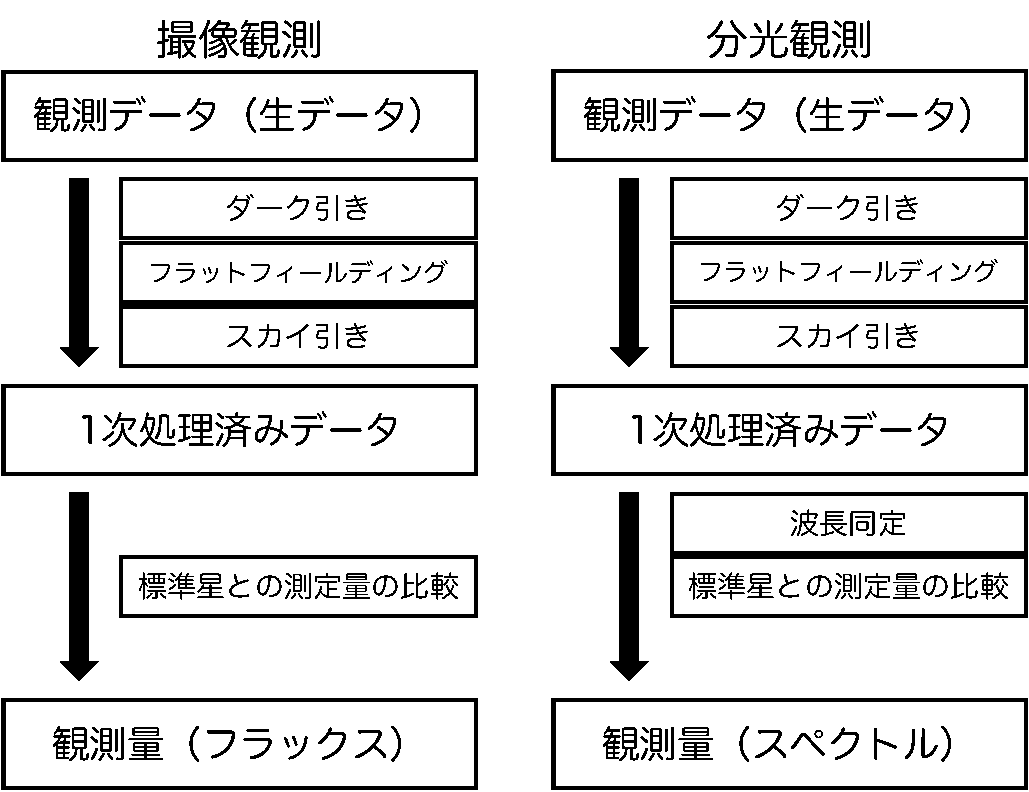
\includegraphics[width=0.7\linewidth]{./fig/chap_5/photo_spec.pdf}
	\caption{撮像/分光観測データの解析の流れ}
  \label{fig:kaiseki_nagare}
\end{figure}
\ref{chap:fandamentals_of_observations}~章の流れに則って得られた観測データのことを、ここでは\textbf{生データ}と呼ぶことにします。生データに自分の欲しい天体からの光だけが入っていれば苦労することはないのですが、\textbf{検出機由来の雑音}や\textbf{夜光}などの影響を受けています。図~\ref{fig:initial_reduction}がそれを模式的に表したものです。
\begin{figure}
  \centering
	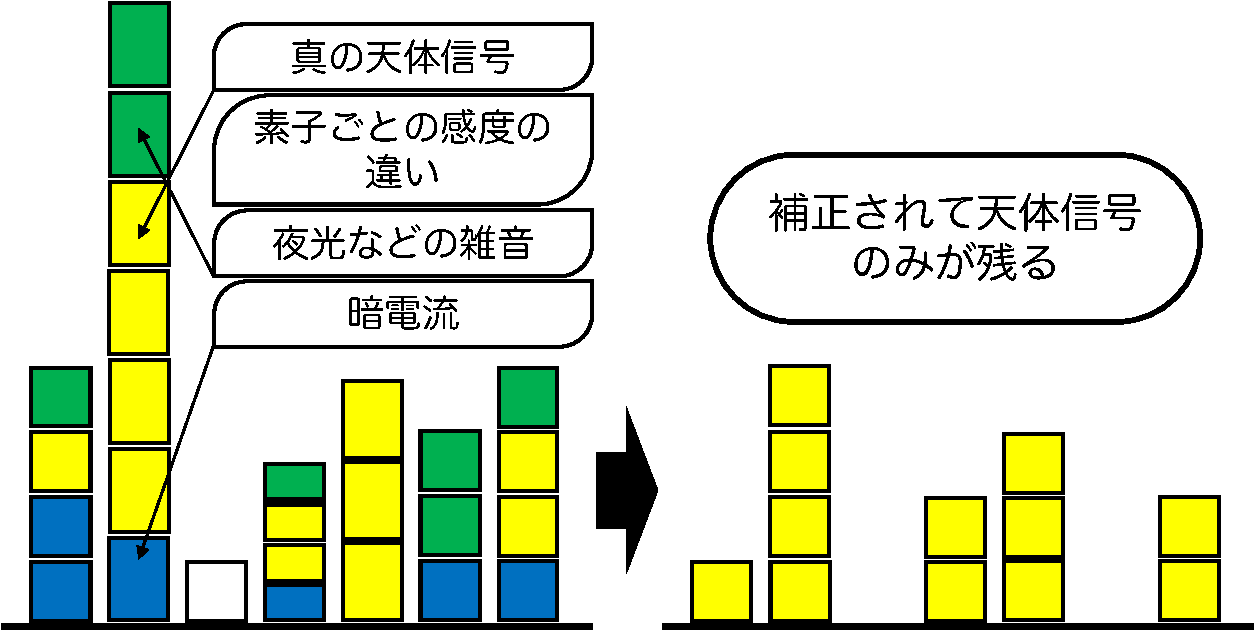
\includegraphics[width=0.7\linewidth]{./fig/chap_5/initial_reduction.pdf}
	\caption[1次処理の仕組み]{1次処理の仕組み。黄色が天体からの光、青が暗電流(ダーク)、緑がスカイ成分を表す。また、大きさの違いは検出機の素子の感度が場所によって異なることを表し、色がついていないのはその素子が死んでいることを表す。このような、観測したい天体のみの情報を使って議論をしたいにも関わらず、混ざってしまう雑音などを取り除く作業が1次処理である。}
  \label{fig:initial_reduction}
\end{figure}
実際に式的にその影響を表すと
\begin{align}
  (\text{生データ}) =  (\text{感度の違い}) \times \left\{  (\text{真の天体信号})+(\text{暗電流})+(夜光などの雑音) \right\}\label{eq:nama_data}
\end{align}
のようになります。\par
\textbf{暗電流}とは、検出機が温度を持っていることで流れてしまう電子雑音のことです。天体放射の検出の仕組みは大まかに
\begin{align*}
  (\text{天体からの光子}) \xrightarrow{\text{検出器}} (\text{光電効果による電子}) \rightarrow (\text{光電流の発生})
\end{align*}
となっています。この二つ目の段階で、天体放射やその他の雑音に加えて、熱雑音による電流が加わります。
これを「\textbf{暗電流}」と呼びます。
この雑音は単純に検出器を冷やせば減らすことができます。
実際、赤外線検出器は$-76\,\mathrm{{}^\circ C}$、市販の可視光の検出器は$-10\,\mathrm{{}^\circ C}$に冷やして使われています。
しかし、天体からの放射がわからなくなるほどの雑音の影響を軽減することはできても、完全に$0$にすることは不可能なため、この成分を引く作業が必要となります。
この作業を「暗電流」が「\textbf{ダーク}」と呼ばれることから、「\textbf{ダーク引き}」と呼びます。\par
CCDカメラなどの検出機は、多数の素子によって構成されていますが、望遠鏡や、付属する検出器を合わせた系の、光子検出に対する感度は必ずしも一様ではありません。とても強く光子に対して反応する素子も存在する一方で、全く反応しない、「死んだ素子」も存在します。このような感度の違いを補正する処理を\textbf{フラットフィールディング}と呼びます。\par
「\textbf{夜光などの雑音}」とはその名の通り、夜光や大気による雑音の成分です。今回考える主な成分は
\begin{itemize}
  \item 主にKバンドより長い波長で、大気や望遠鏡の熱的な放射成分を見てしまう$(\sim300\,\mathrm{K})$
  \item 主にHバンドで、OH夜光の輝線成分によるフリンジパターン
\end{itemize}
です。これを以降は「\textbf{スカイ}」と呼び、スカイを引く補正のことを、「\textbf{スカイ引き}」と呼ぶことにします。\par
これらの補正のことをまとめて\textbf{1次処理}と呼びます。撮像、分光のどちらでもこの処理が必要になりますが、分光はまとめてIRAFでやってしまった方が楽なので、撮像ではPython、分光ではIRAFを使った処理を行い、観測量を得るにはどうすればよいかをまとめていきます。

\section{撮像データ解析} %%
\label{sect:photo_ana}
今回サンプルとして扱うデータは以下のURLに置いてあります。
\begin{verbatim}
  https://drive.google.com/drive/folders/1ZGkWFySTgc-MVdViP_U_AfD8XPUrSbWi
\end{verbatim}

中身は次のようになっています。\texttt{raw}が天体を撮像した生データ、\texttt{flat}がフラットフィールディングに用いるデータ、\texttt{dark}がダーク引きで用いるデータです。
\begin{verbatim}
  dark % ls
  ir0029.fits   ir0030.fits   ir0031.fits   ir0032.fits   ir0033.fits
  flat % ls
  ir0006.fits   ir0007.fits   ir0008.fits   ir0009.fits   ir0010.fits
  raw % ls
  ir0011.fits   ir0012.fits   ir0013.fits   ir0014.fits   ir0015.fits
  ir0016.fits   ir0017.fits   ir0018.fits   ir0019.fits
\end{verbatim}

また、解析コードとして\texttt{initial\_data\_reduction.py}と\texttt{photometry.py}が付属しています。まずは\texttt{initial\_data\_reduction.py}の内容を扱います。\par
解析にさきだって、今回扱う生データを見てみましょう。図~\ref{fig:raw_data}です。
\begin{figure}
	\centering
	\subfigure[]{%
	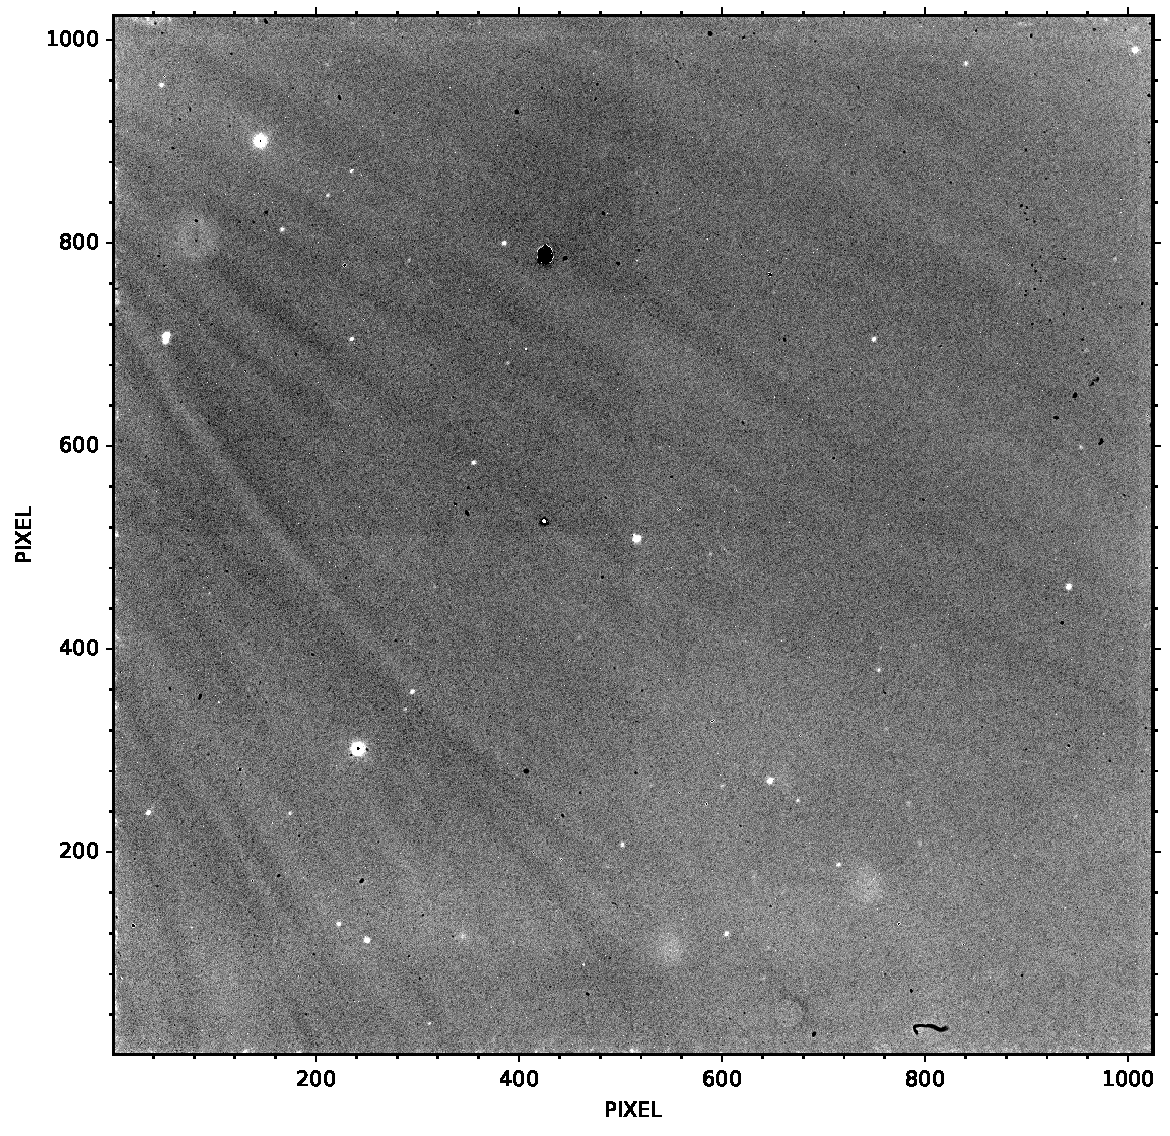
\includegraphics[width=.333\textwidth,clip]{./fig/chap_5/fig_ir_00.pdf}%
	\label{fig:raw_figs_0}%
	}%
	\subfigure[]{%
	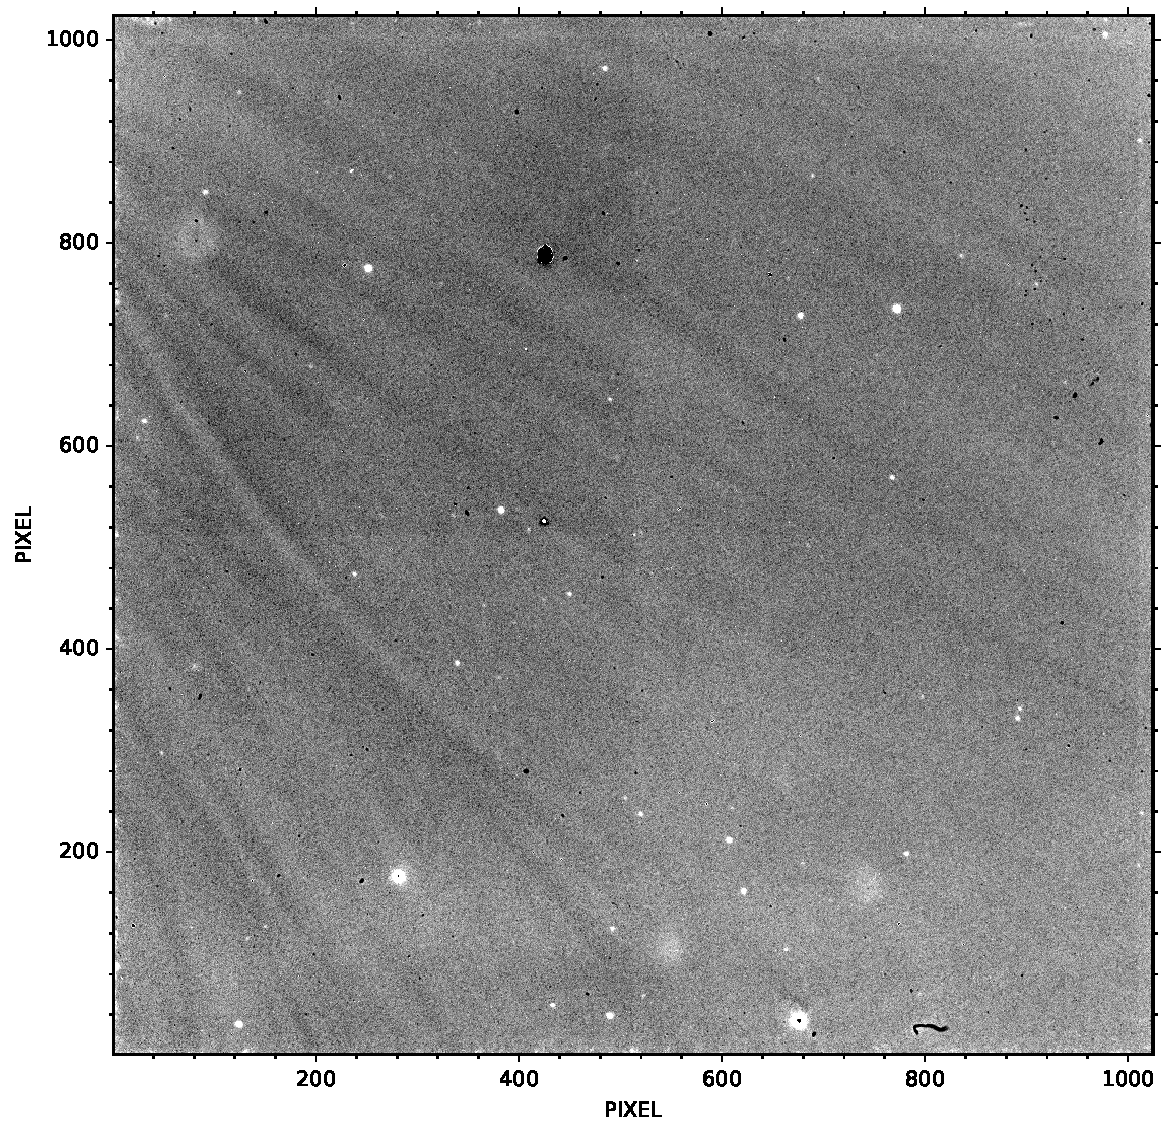
\includegraphics[width=.333\textwidth,clip]{./fig/chap_5/fig_ir_01.pdf}%
	\label{fig:raw_figs_1}%
	}%
  \subfigure[]{%
	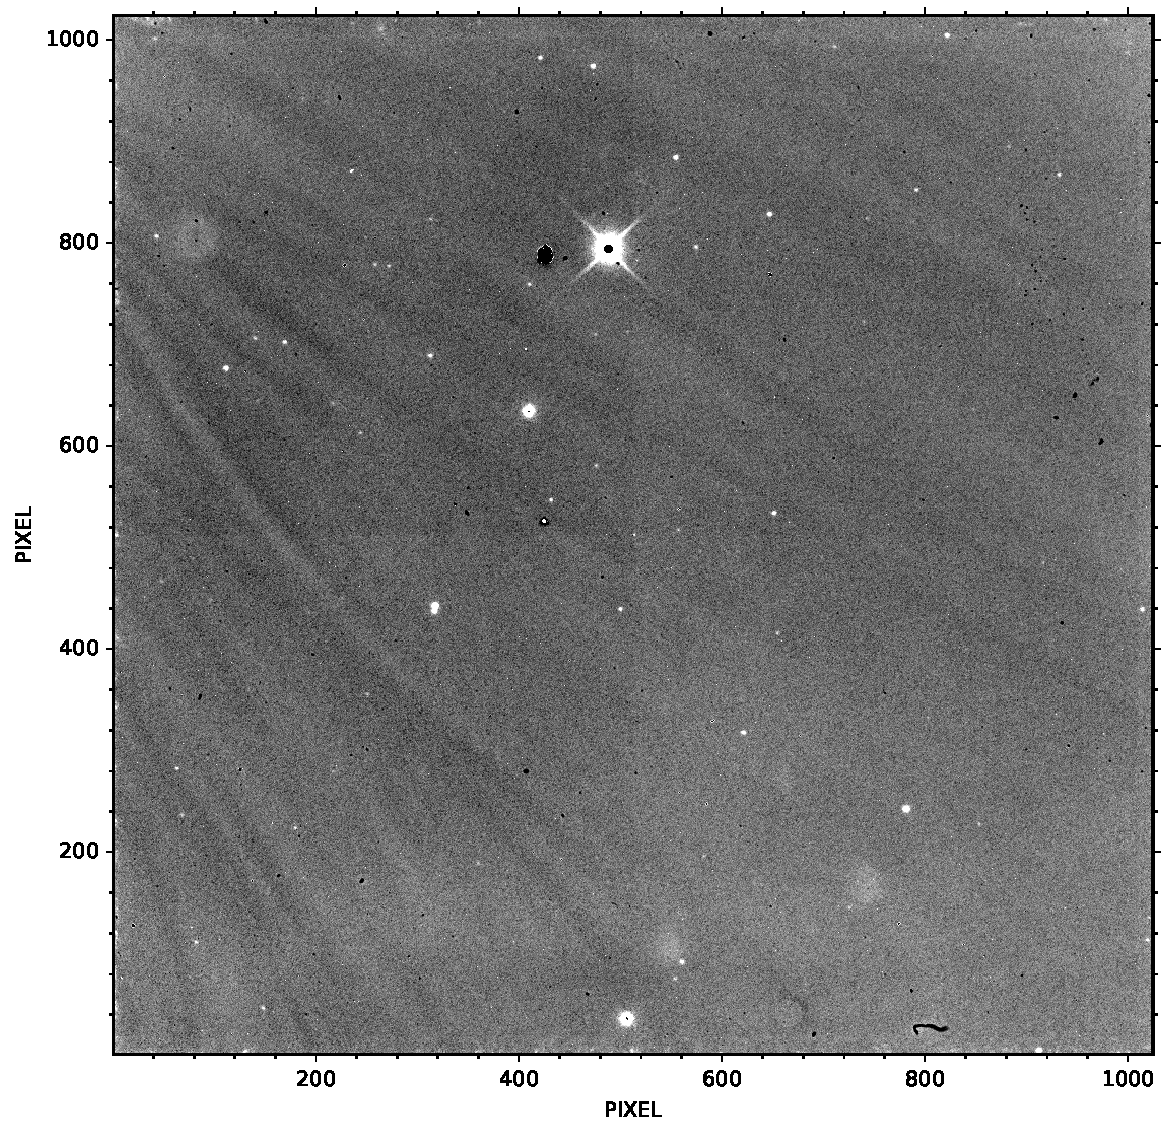
\includegraphics[width=.333\textwidth,clip]{./fig/chap_5/fig_ir_02.pdf}%
	\label{fig:raw_figs_2}%
	}
  \subfigure[]{%
	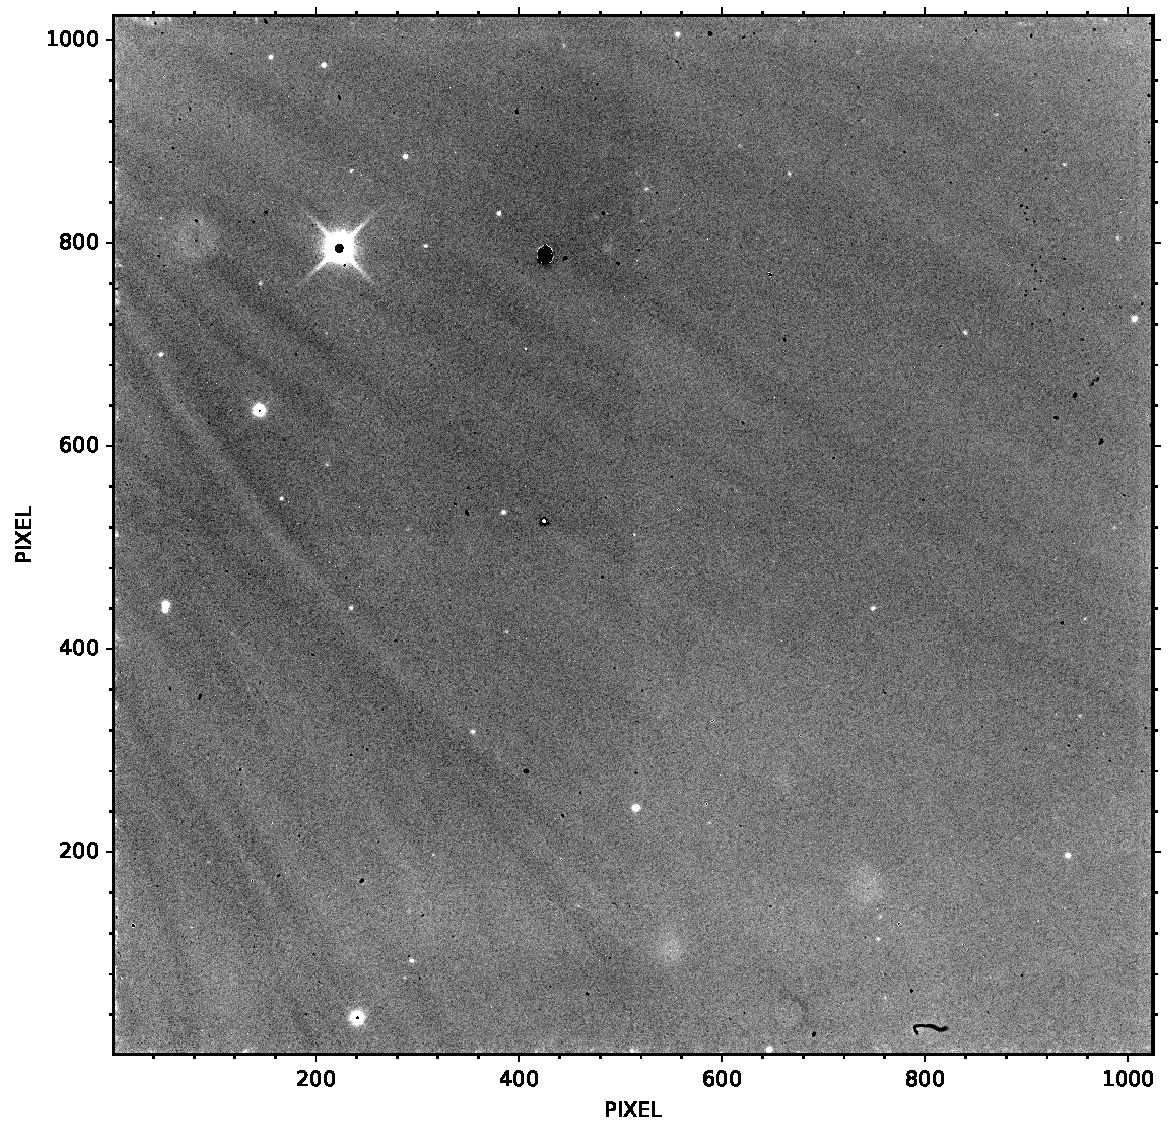
\includegraphics[width=.333\textwidth,clip]{./fig/chap_5/fig_ir_03.pdf}%
	\label{fig:raw_figs_3}%
	}%
	\subfigure[]{%
	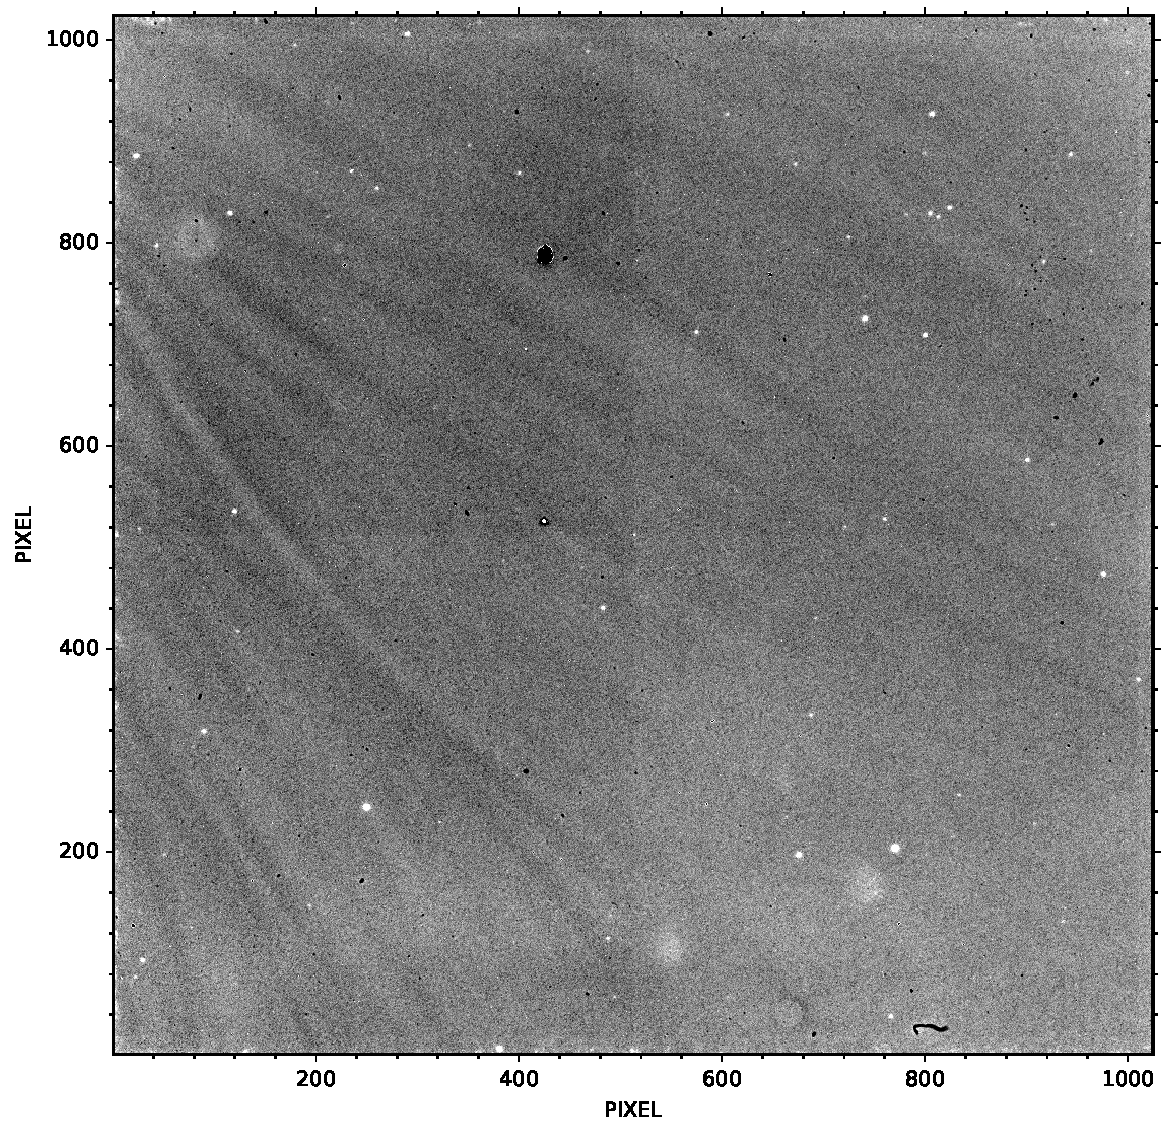
\includegraphics[width=.333\textwidth,clip]{./fig/chap_5/fig_ir_04.pdf}%
	\label{fig:raw_figs_4}%
	}%
  \subfigure[]{%
	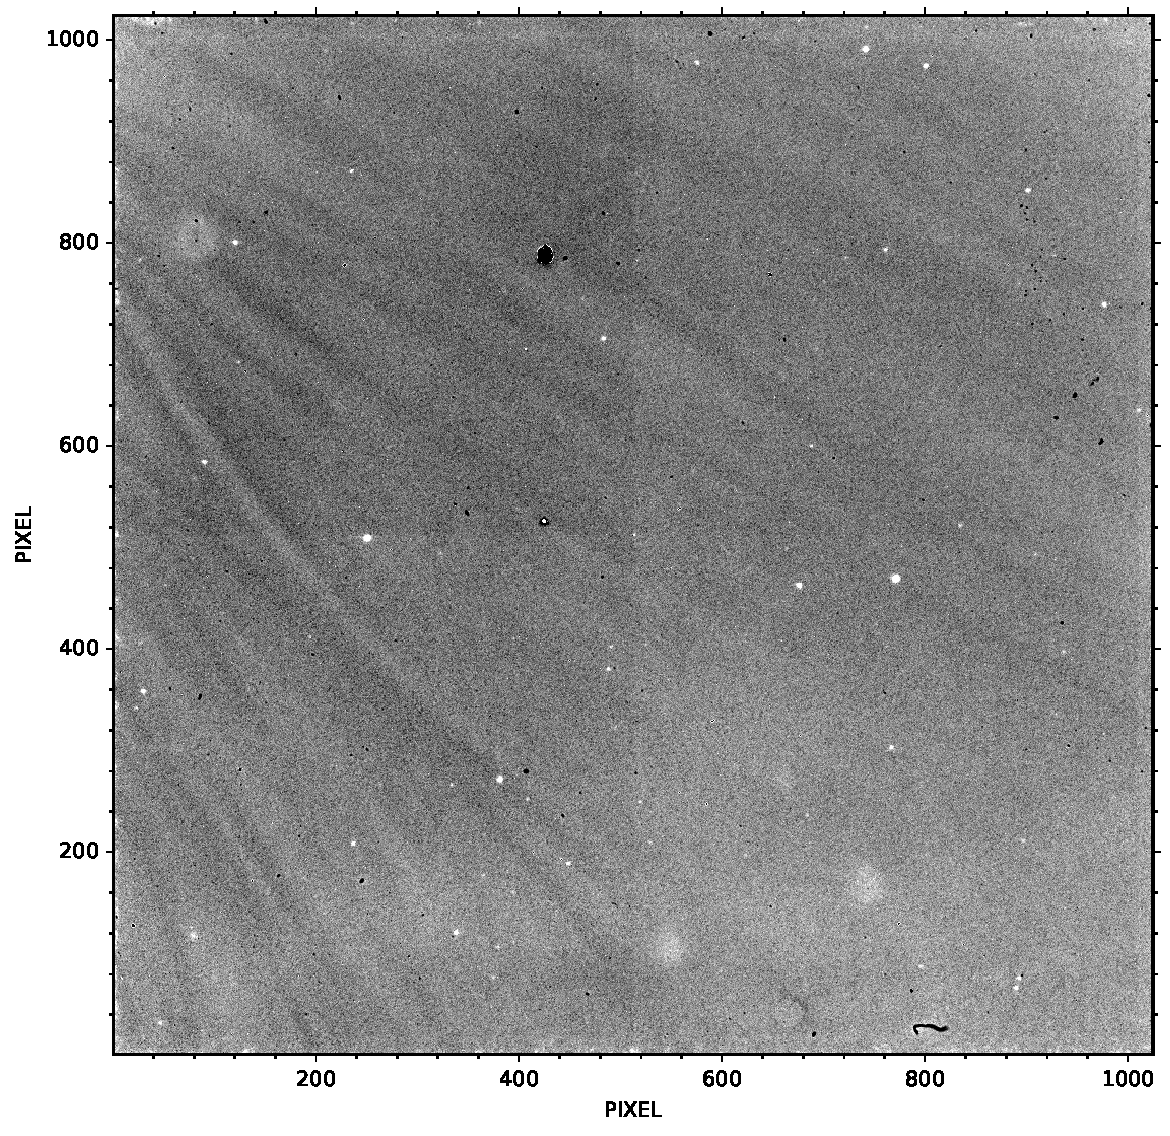
\includegraphics[width=.333\textwidth,clip]{./fig/chap_5/fig_ir_05.pdf}%
	\label{fig:raw_figs_5}%
	}
  \subfigure[]{%
	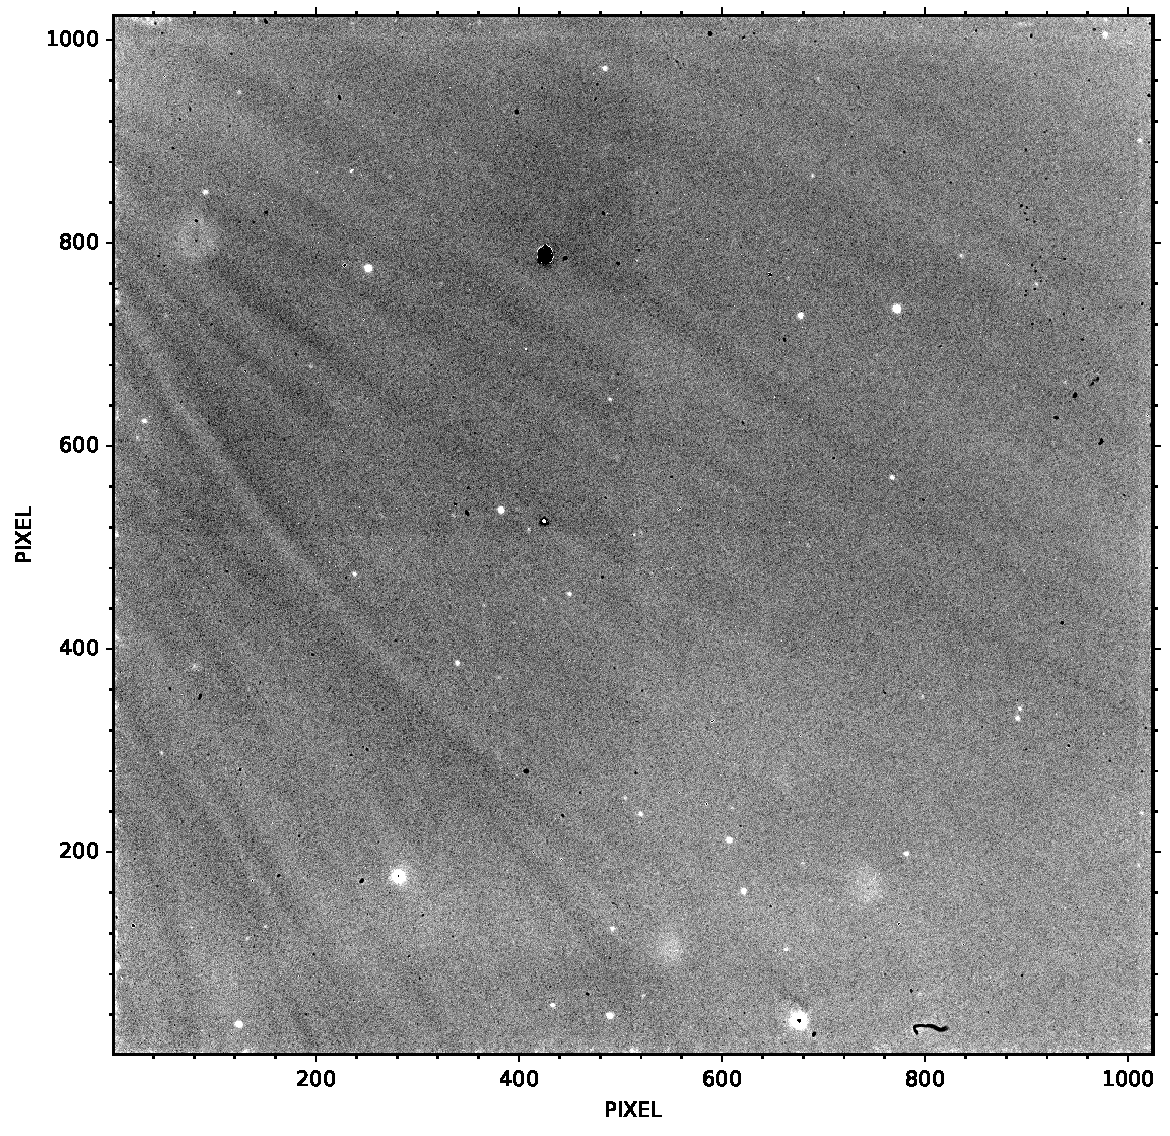
\includegraphics[width=.333\textwidth,clip]{./fig/chap_5/fig_ir_06.pdf}%
	\label{fig:raw_figs_6}%
	}%
	\subfigure[]{%
	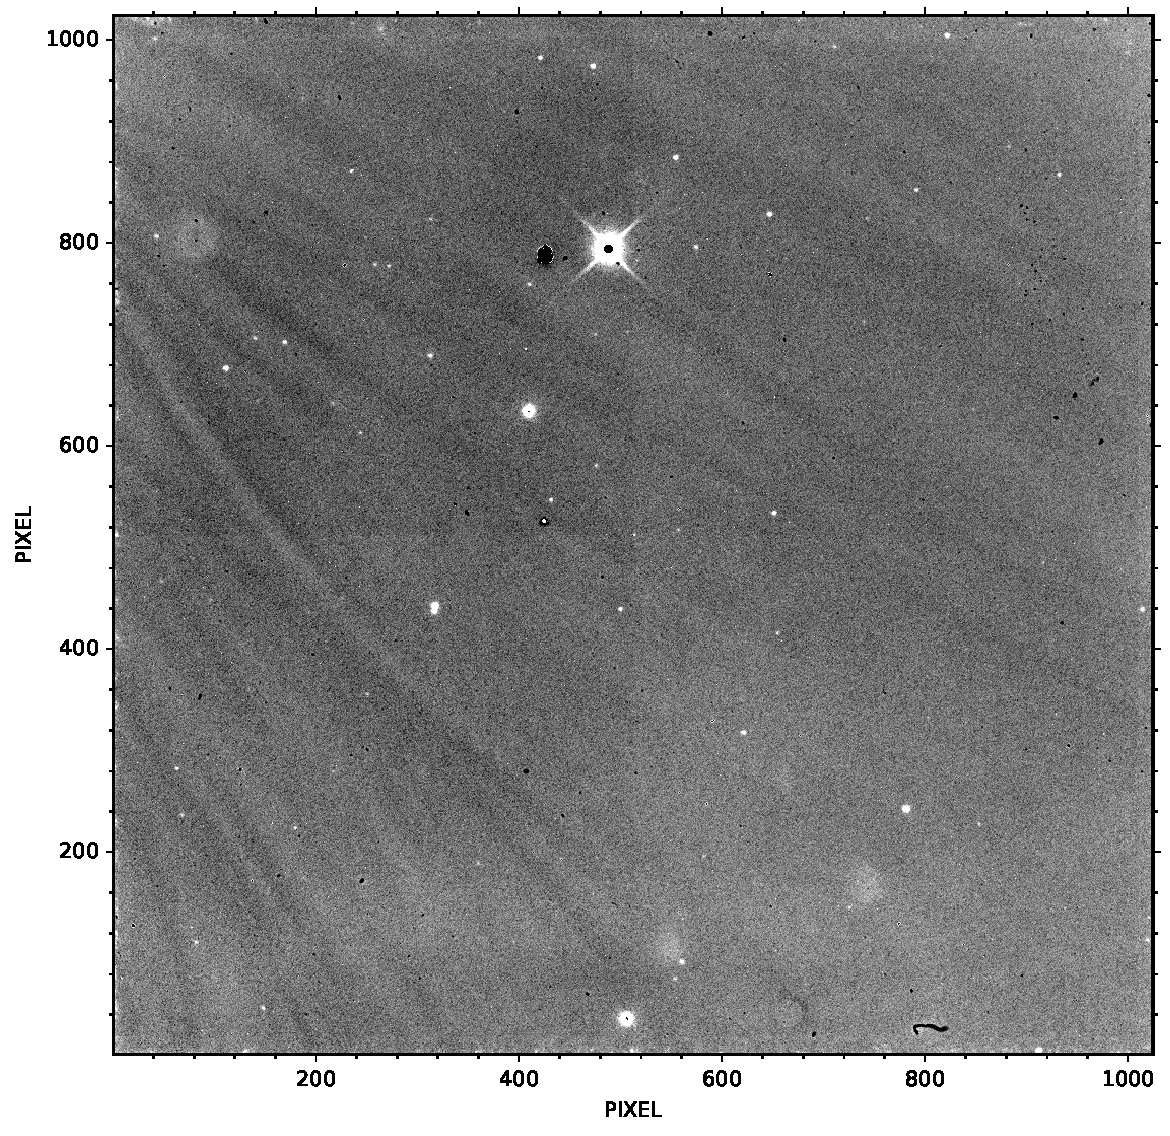
\includegraphics[width=.333\textwidth,clip]{./fig/chap_5/fig_ir_07.pdf}%
	\label{fig:raw_figs_7}%
	}%
  \subfigure[]{%
	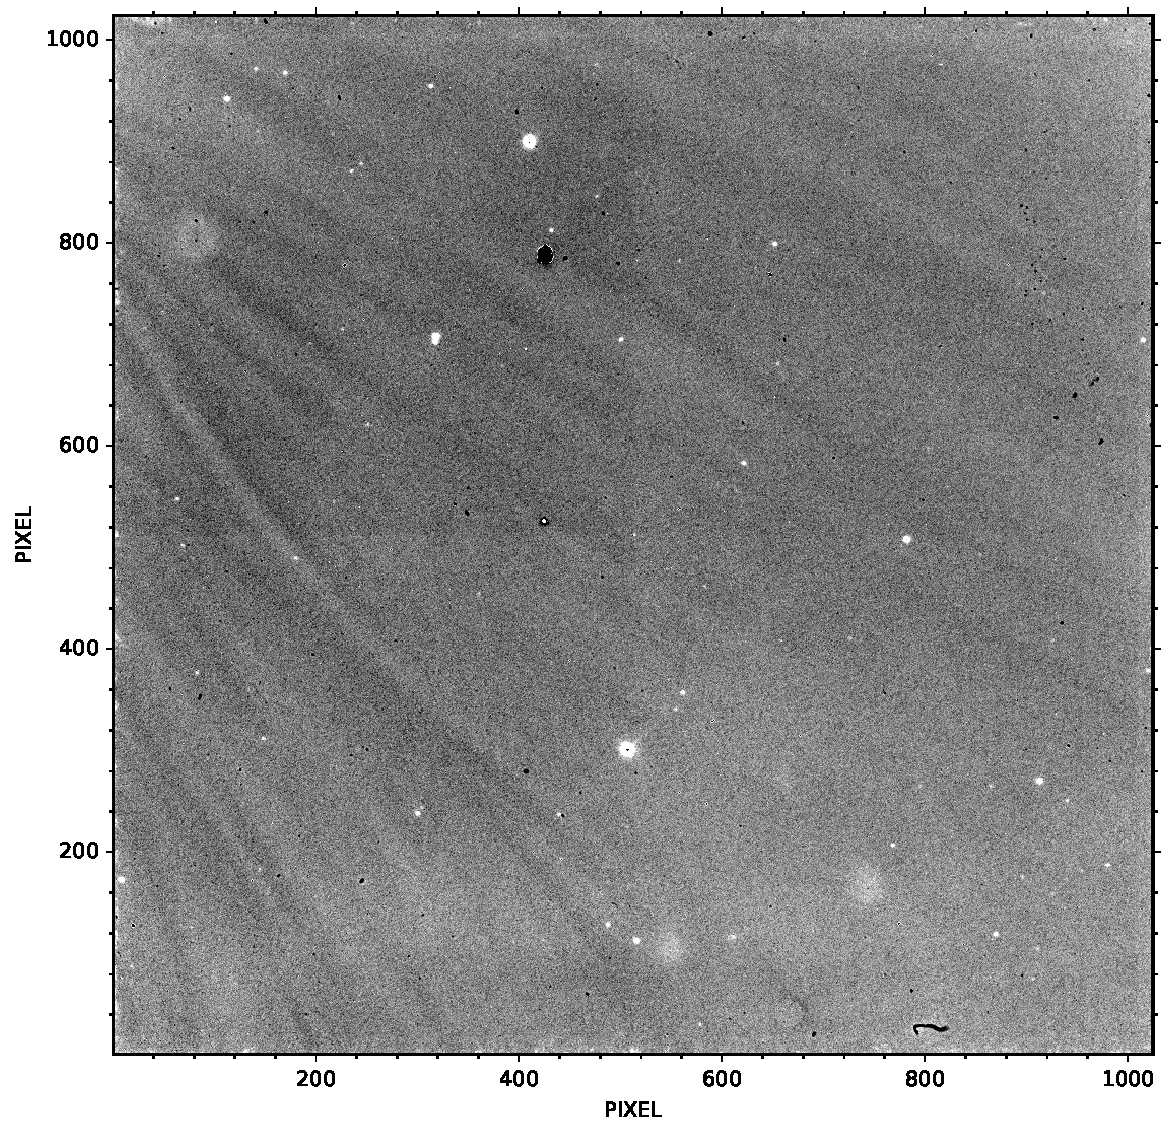
\includegraphics[width=.333\textwidth,clip]{./fig/chap_5/fig_ir_08.pdf}%
	\label{fig:raw_figs_8}%
	}
	\caption{生データ画像}
	\label{fig:raw_data}
\end{figure}
星のようなものが写ってはいますが、あまり綺麗とは言えない状態です。これは先ほど述べた様々な雑音などの成分の影響を受けているためです。これから行う処理によって綺麗な画像にしていきます。

\subsubsection{コードの実行の仕方}
ここではPythonやその他言語の扱いに慣れていない方のために、Pythonのコード実行の仕方を説明します。慣れている方はそのまま読み飛ばしてください。

\subsubsection{バイアス引き}
実際の作業に入る前に、「\textbf{バイアス引き}」について解説します。バイアスとは、人為的にデータに足されている量です。これは、本来観測で得られる出力値が、不良素子の影響で負になることを防ぐために足される一定値です。この値を調べるためには、「露出$0$秒」で画像を撮れば良いことになります。しかし、これはダークの成分にも含まれているので、ダークを引けばバイアスを引いたことにもなりますから、この作業は\textbf{必要ありません}。

\subsubsection{ダーク引き}
「\textbf{ダーク}」はカメラのシャッター、または望遠鏡の蓋を閉じた状態で、\textbf{天体の露出時間と同じ時間撮影を行う}ことによって出力されるものです。実際、ダークがどんな画像なのかをみてみましょう。\par
まずは準備として、必要なモジュールをimportします。次のコードを実行してください。
\begin{lstlisting}[caption=モジュールのimport, label=code:import]
  import os
  import re
  import numpy as np
  import astropy.io.fits as fits
  import glob
  import matplotlib.pyplot as plt
  import aplpy

  # create a directory if that directory does not exist
  def my_makedirs(path):
      if not os.path.isdir(path):
          os.makedirs(path)
  my_makedirs('./out')


  # functions for the function "sorted()"
  def atoi(text):
      return int(text) if text.isdigit() else text
  def natural_keys(text):
      return [ atoi(c) for c in re.split(r'(\d+)', text) ]
\end{lstlisting}
\texttt{import}から始まる文が今回の1次処理で使用するモジュール類です。また、引数として取った文字列を名前として持つディレクトリが存在しない場合に、ディレクトリを作成する関数\texttt{my\_makedirs}を作り、\texttt{out}というディレクトリを作成しました。これから出力される\texttt{.fits}ファイルは全てここに保存するようにします。\par
また、\texttt{sorted}という関数をこの後に使用するため、この関数を使用するのに必要な関数を2つ定義しています。\par
次にダーク画像を作成します。ダークは複数回撮ることが一般的なので、それらを全て結合する必要があります。今回は5枚とってあるので、それらを結合します。処理としては次のようになります。
\begin{lstlisting}[caption=ダーク画像の作成, label=code:mk_dark]
  # dark
  ## merge the dark images
  dark_images = np.empty((0, 1024, 1024))
  dark_fits = sorted(glob.glob('./dark/*.fits'), key=natural_keys)
  for data in dark_fits:
      dark = fits.getdata(data)
      dark_images = np.append(dark_images, dark[np.newaxis, :], axis=0)

  median_dark = np.median(dark_images, axis=0)
  fits.writeto('./out/dark.fits', median_dark, overwrite=True)
\end{lstlisting}
ここでの流れは次のようになっています。
\begin{enumerate}[(1)]
  \item 1024$\times$1024$\times$0の3次元の画像を用意
  \item 今回扱うダークの\texttt{fits}を全て取得
  \item 取得したダーク\texttt{fits}でループ処理
  \begin{itemize}
    \item データを一つずつ取得してその中央値をとる
  \end{itemize}
  \item できた画像を保存
\end{enumerate}

できた\texttt{fits}形式のファイルを表示してみます。下のコードを実行すると、図~\ref{fig:dark}が\texttt{fig}というフォルダの中にあるはずです。
\begin{lstlisting}[caption=ダーク画像の表示, label=code:dark]
  my_makedirs('./fig')

  img = fits.open('./out/dark.fits')
  pic = aplpy.FITSFigure(img)
  pic.show_grayscale()
  pic.save('./fig/dark_fits.pdf')
\end{lstlisting}
\begin{figure}
  \centering
	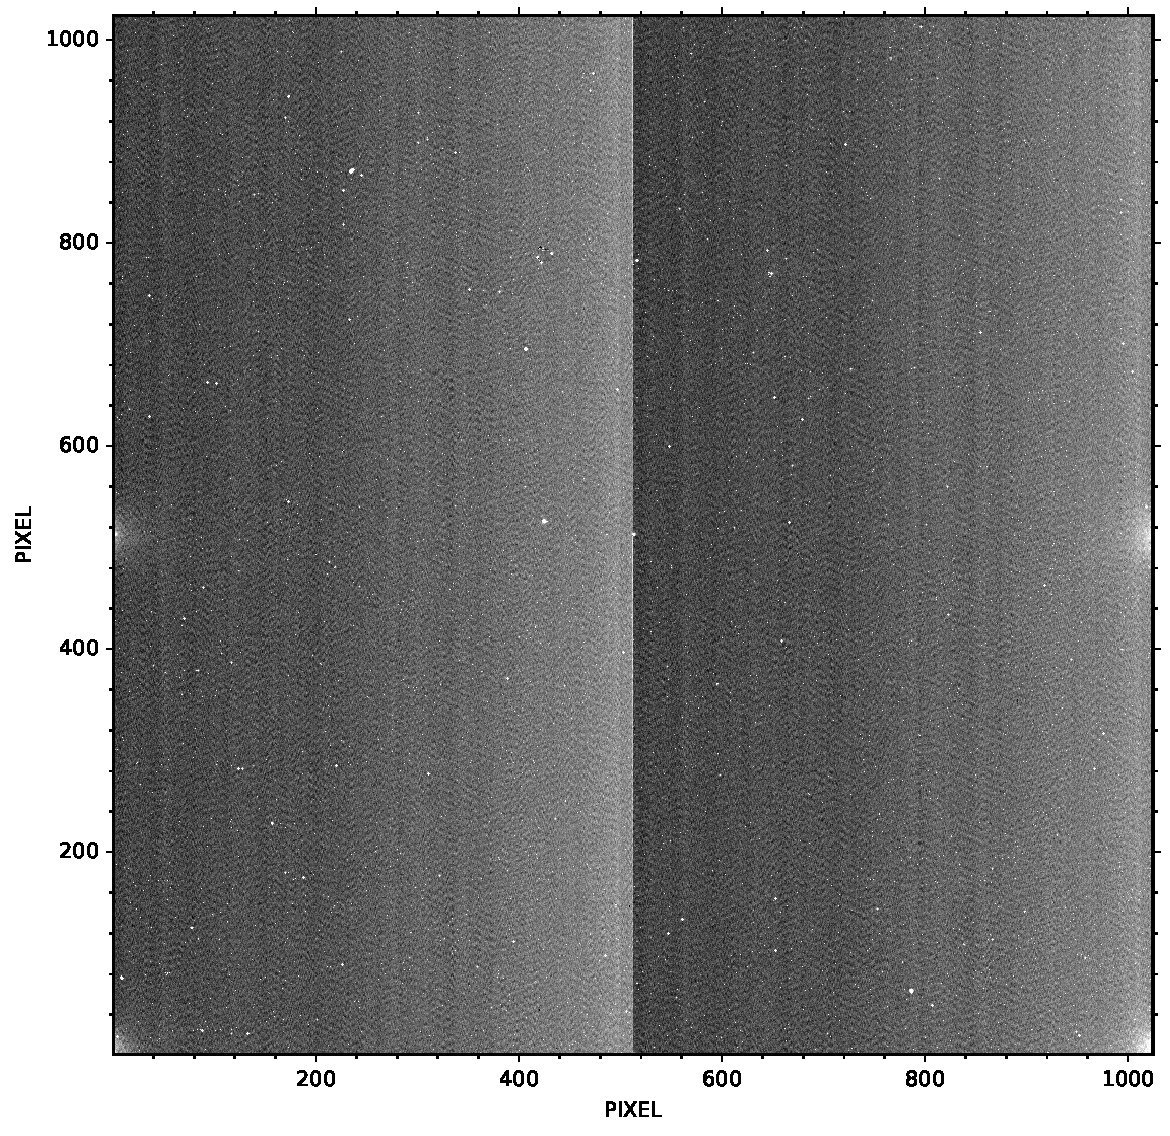
\includegraphics[width=0.6\linewidth]{./fig/chap_5/dark_fits.pdf}
	\caption{ダークの結合画像}
  \label{fig:dark}
\end{figure}

明るい点が複数個確認できると思います。これは数理統計で習う、正規分布に従ったノイズの成分で、よく「3$\sigma$ノイズ」だったり、「5$\sigma$ノイズ」と読んだりします。この$\sigma$は標準偏差の意味です。正規分布表と調べたりすると出てくるので、適宜調べて欲しいのですが、3$\sigma$は大体$1/1000$の確率で発生する事象ということになります。今回のダークや天体画像のピクセル数は$1024\times1024$で、$10^{6}$のオーダーなので、1枚の画像に$1000$の、リアルでないノイズが存在することになります。$5\sigma$であれば大体$1/100000$なので、$10$個くらいです。\par
この\textbf{ダーク}を\textbf{生データ}から引きます。
\begin{lstlisting}[caption=生データからダークを引く, label=code:darkhiki]
  ## subtract the dark data from raw data
  dark = fits.getdata('./out/dark.fits')
  raw_fits = sorted(glob.glob('./raw/*.fits'), key=natural_keys)
  for i,data in enumerate(raw_fits):
      raw_image = fits.getdata(data)
      sub_dark = raw_image - dark
      file_name = 'dir_' + str('{:02d}'.format(i)) + '.fits'
      fits.writeto('./out/' + file_name, sub_dark, overwrite=True)
\end{lstlisting}
これによって、ダークによって生まれてしまう成分をデータから引くことができたことになり、式~\eqref{eq:nama_data}的に言えば、これで得られる画像は
\begin{align}
  (\text{感度の違い}) \times \left\{  (\text{真の天体信号})+(夜光などの雑音) \right\}\label{eq:dir_data}
\end{align}
となっているはずです。ここで注意しなければならないのは、ダークにも検出機の素子の感度の違いがのってしまっていることです。できた画像を表示してみます。
\begin{lstlisting}[caption=ダーク引き済み画像の表示, label=code:darked_fig]
  dir_images = sorted(glob.glob('./out/dir_*.fits'), key=natural_keys)
  for i,data in enumerate(dir_images):
      img = fits.open(data)
      pic = aplpy.FITSFigure(img)
      pic.show_grayscale()
      img_name = 'fig_dir_' + str('{:02d}'.format(i)) + '.pdf'
      pic.save('./fig/' + img_name)
\end{lstlisting}
このコードによって作成される画像が図~\ref{fig:darked_figs}です。
\begin{figure}
	\centering
	\subfigure[]{%
	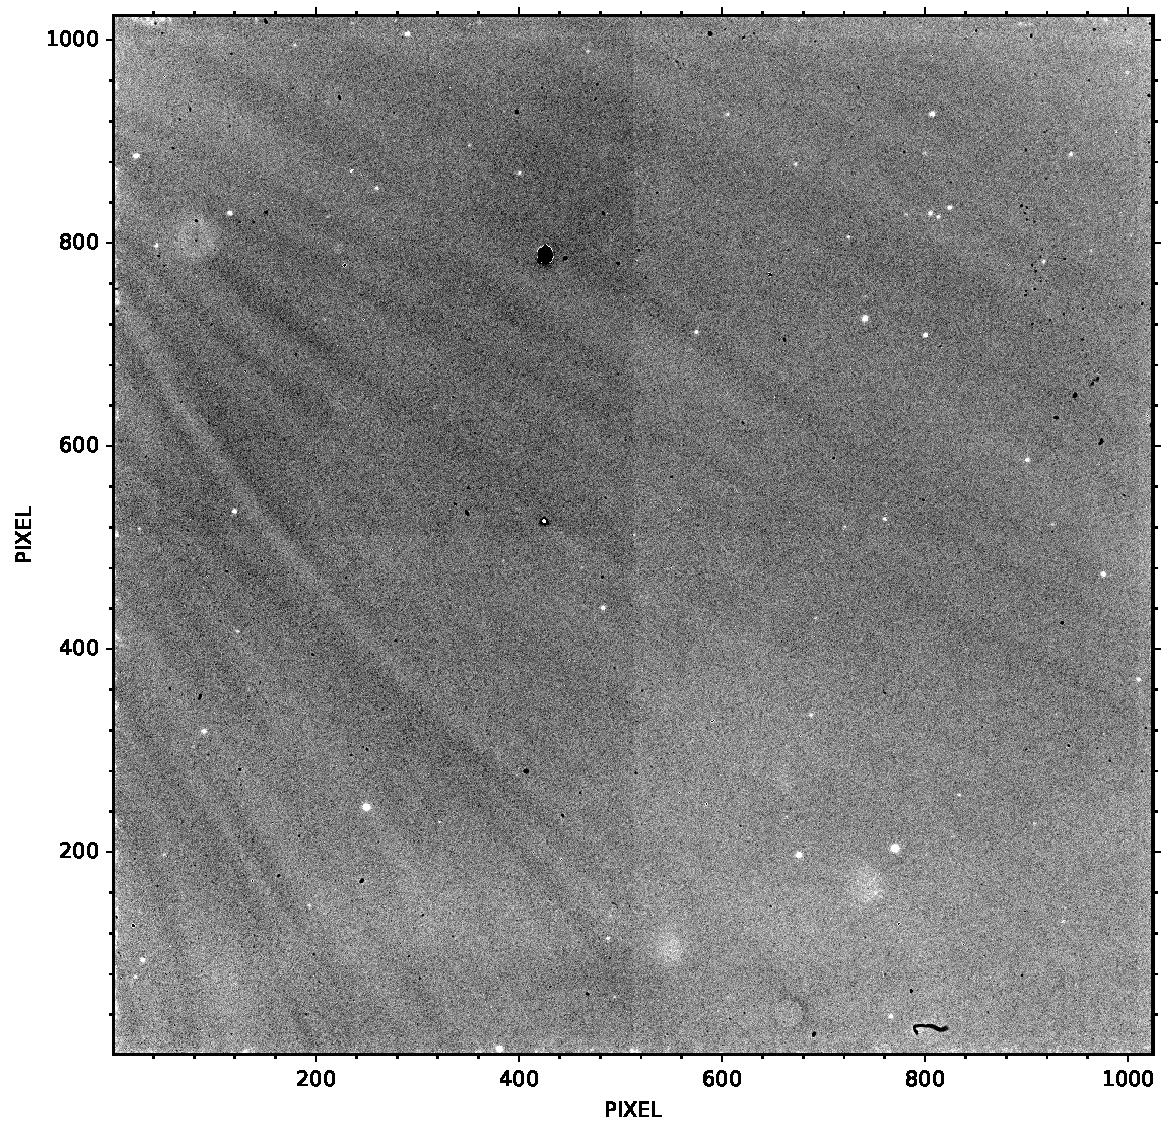
\includegraphics[width=.333\textwidth,clip]{./fig/chap_5/fig_dir_00.pdf}%
	\label{fig:darked_figs_0}%
	}%
	\subfigure[]{%
	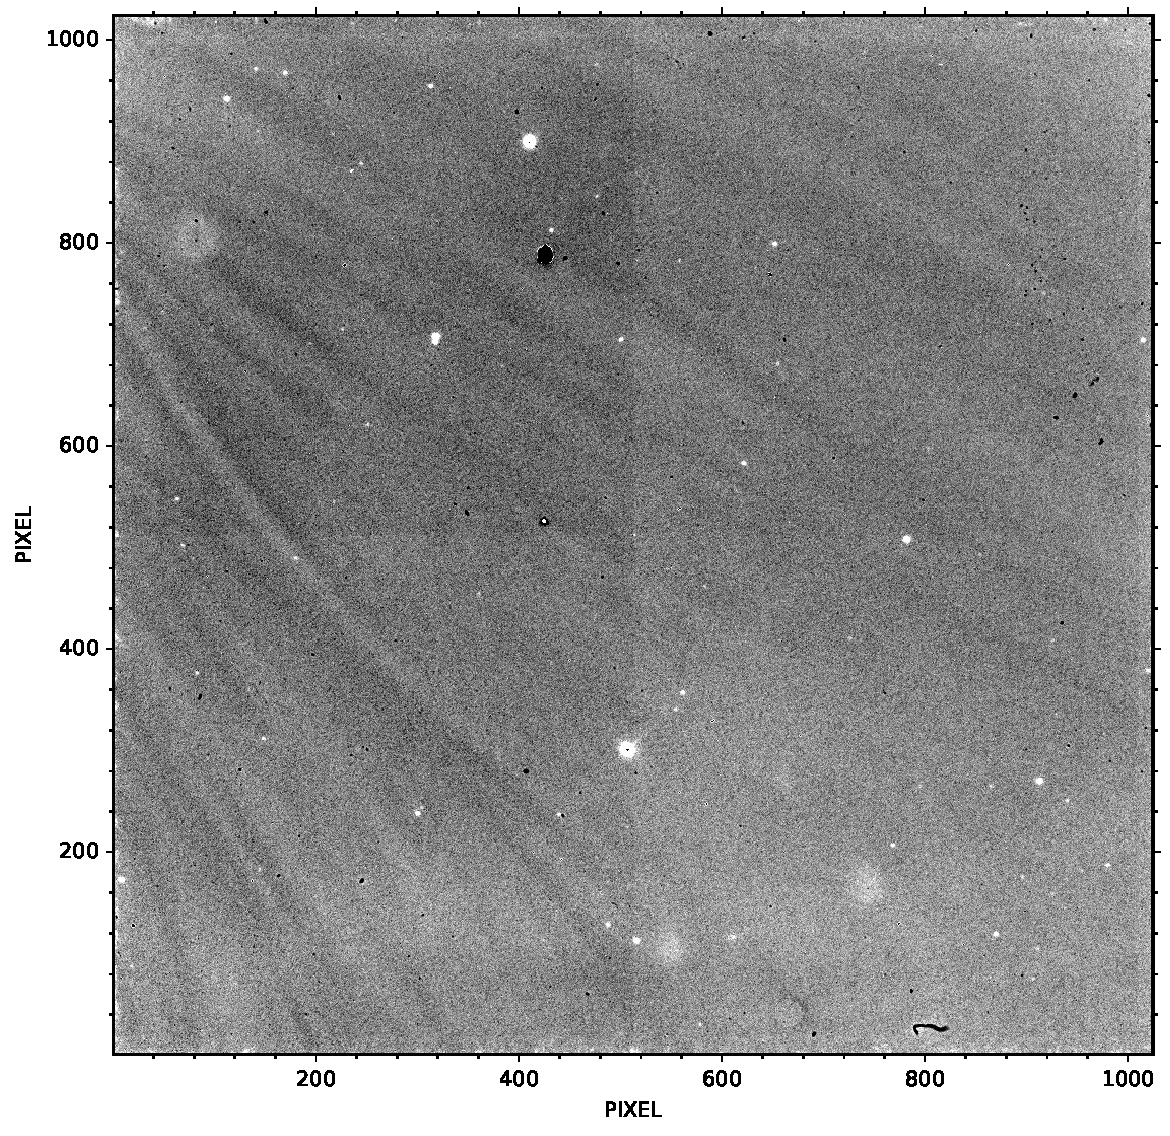
\includegraphics[width=.333\textwidth,clip]{./fig/chap_5/fig_dir_01.pdf}%
	\label{fig:darked_figs_1}%
	}%
  \subfigure[]{%
	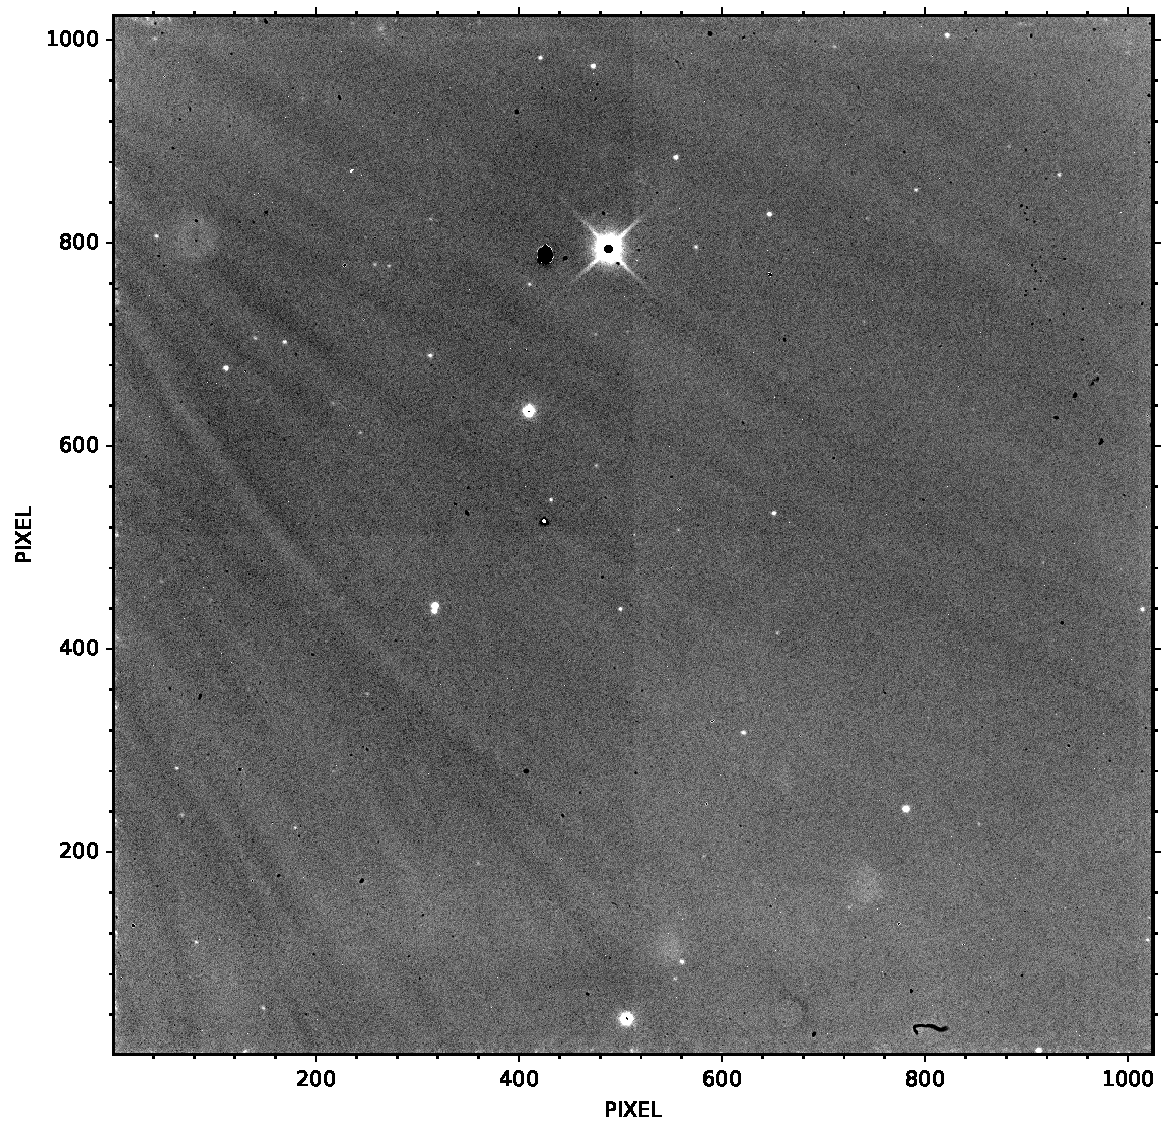
\includegraphics[width=.333\textwidth,clip]{./fig/chap_5/fig_dir_02.pdf}%
	\label{fig:darked_figs_2}%
	}
  \subfigure[]{%
	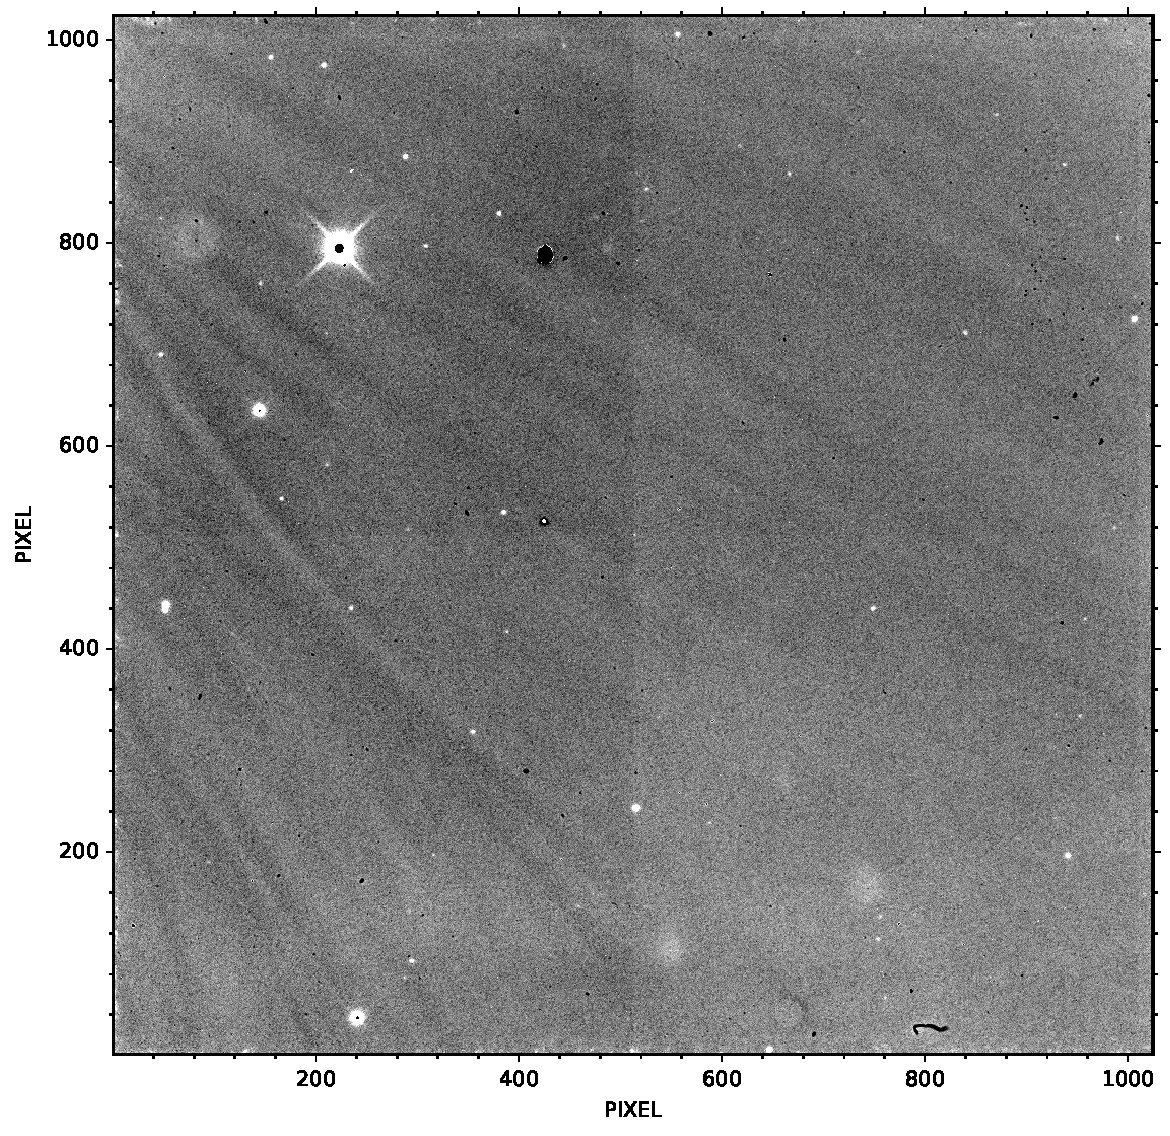
\includegraphics[width=.333\textwidth,clip]{./fig/chap_5/fig_dir_03.pdf}%
	\label{fig:darked_figs_3}%
	}%
	\subfigure[]{%
	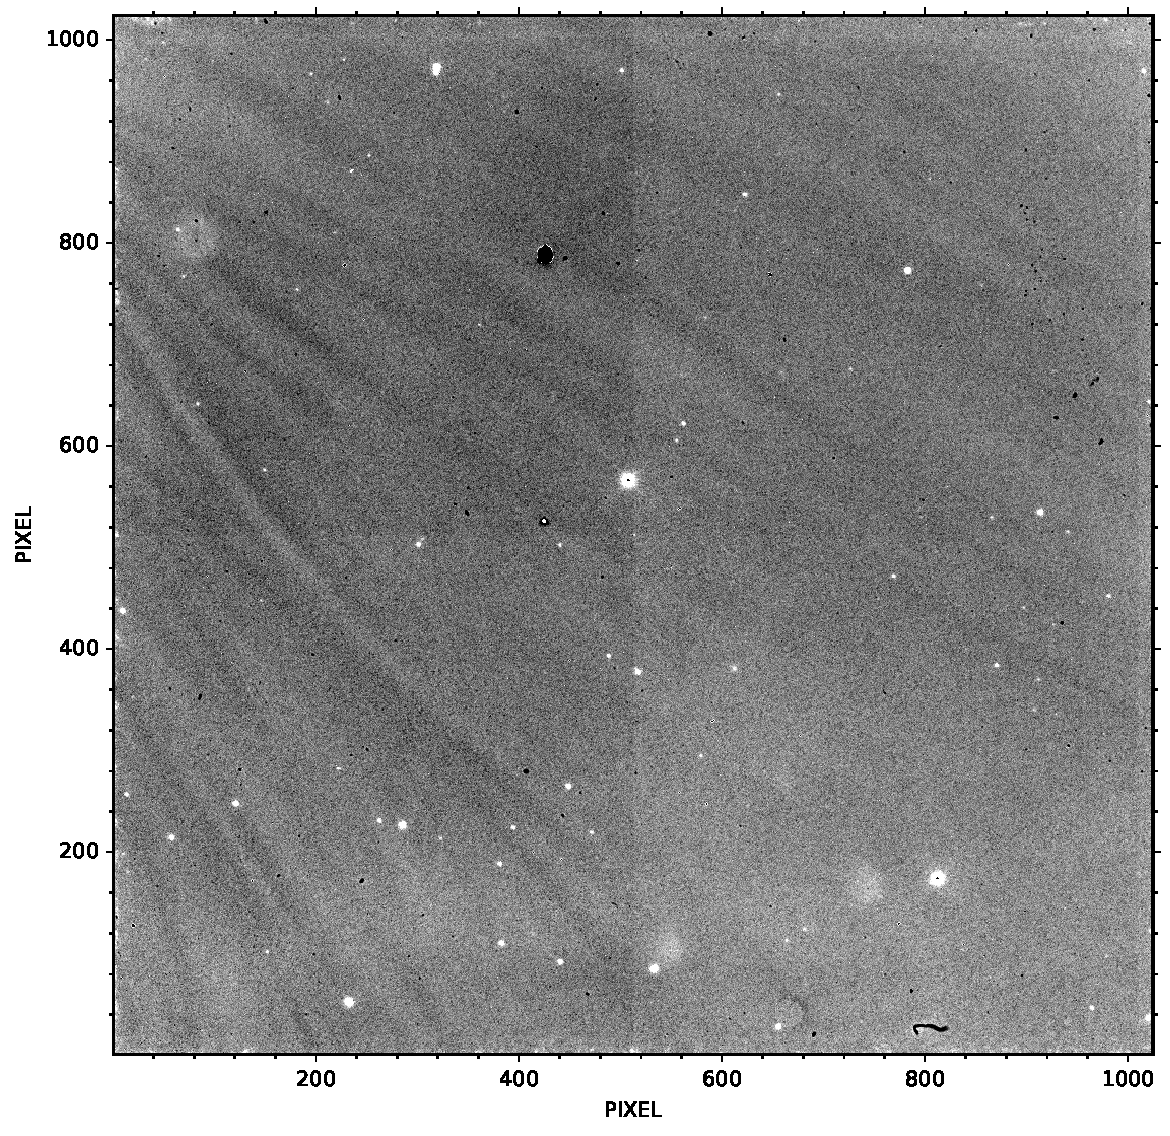
\includegraphics[width=.333\textwidth,clip]{./fig/chap_5/fig_dir_04.pdf}%
	\label{fig:darked_figs_4}%
	}%
  \subfigure[]{%
	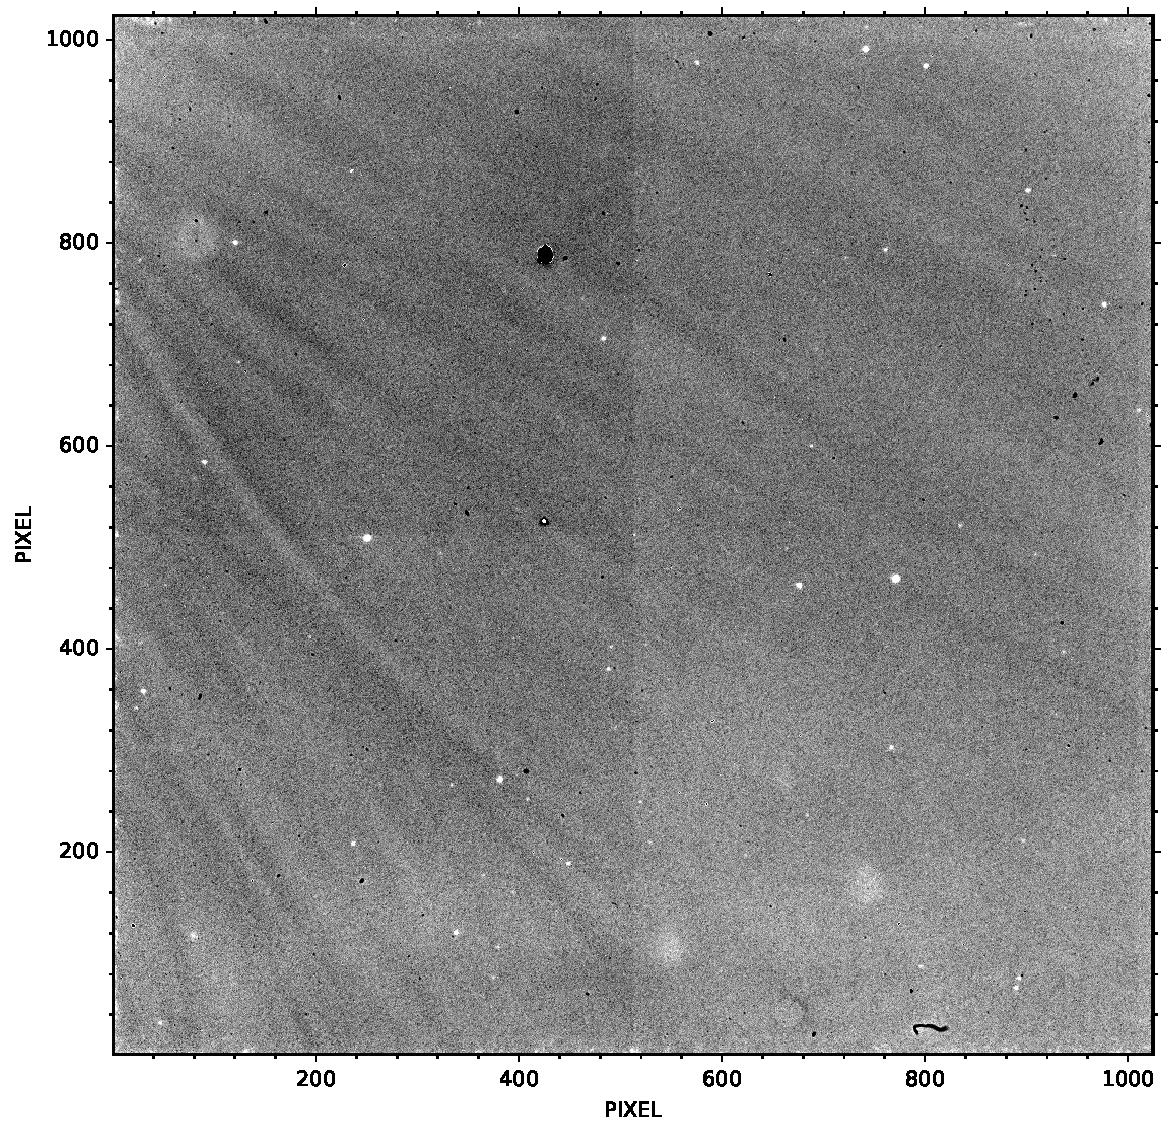
\includegraphics[width=.333\textwidth,clip]{./fig/chap_5/fig_dir_05.pdf}%
	\label{fig:darked_figs_5}%
	}
  \subfigure[]{%
	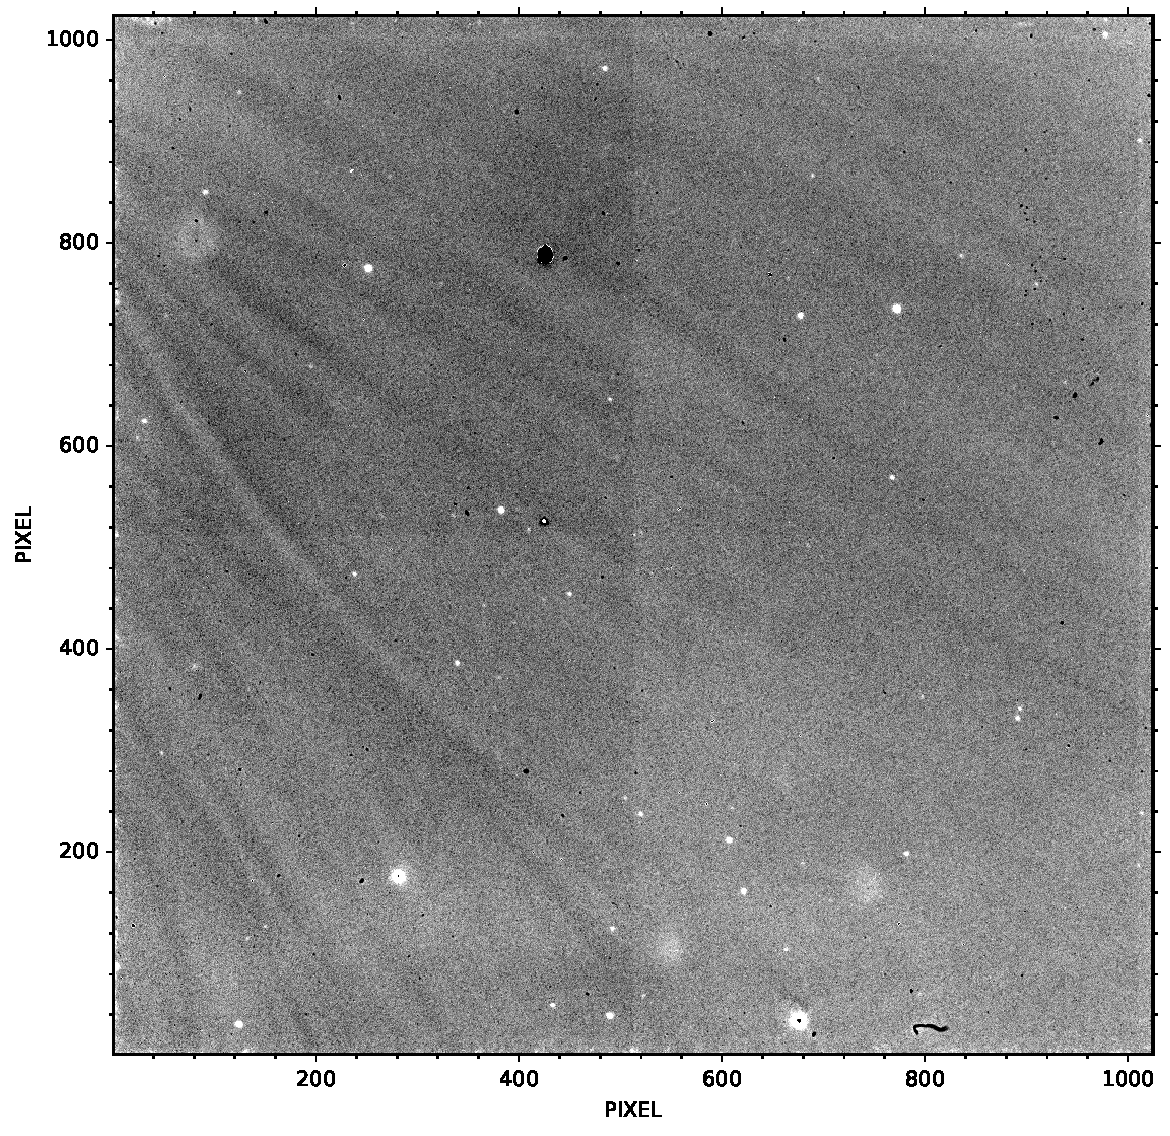
\includegraphics[width=.333\textwidth,clip]{./fig/chap_5/fig_dir_06.pdf}%
	\label{fig:darked_figs_6}%
	}%
	\subfigure[]{%
	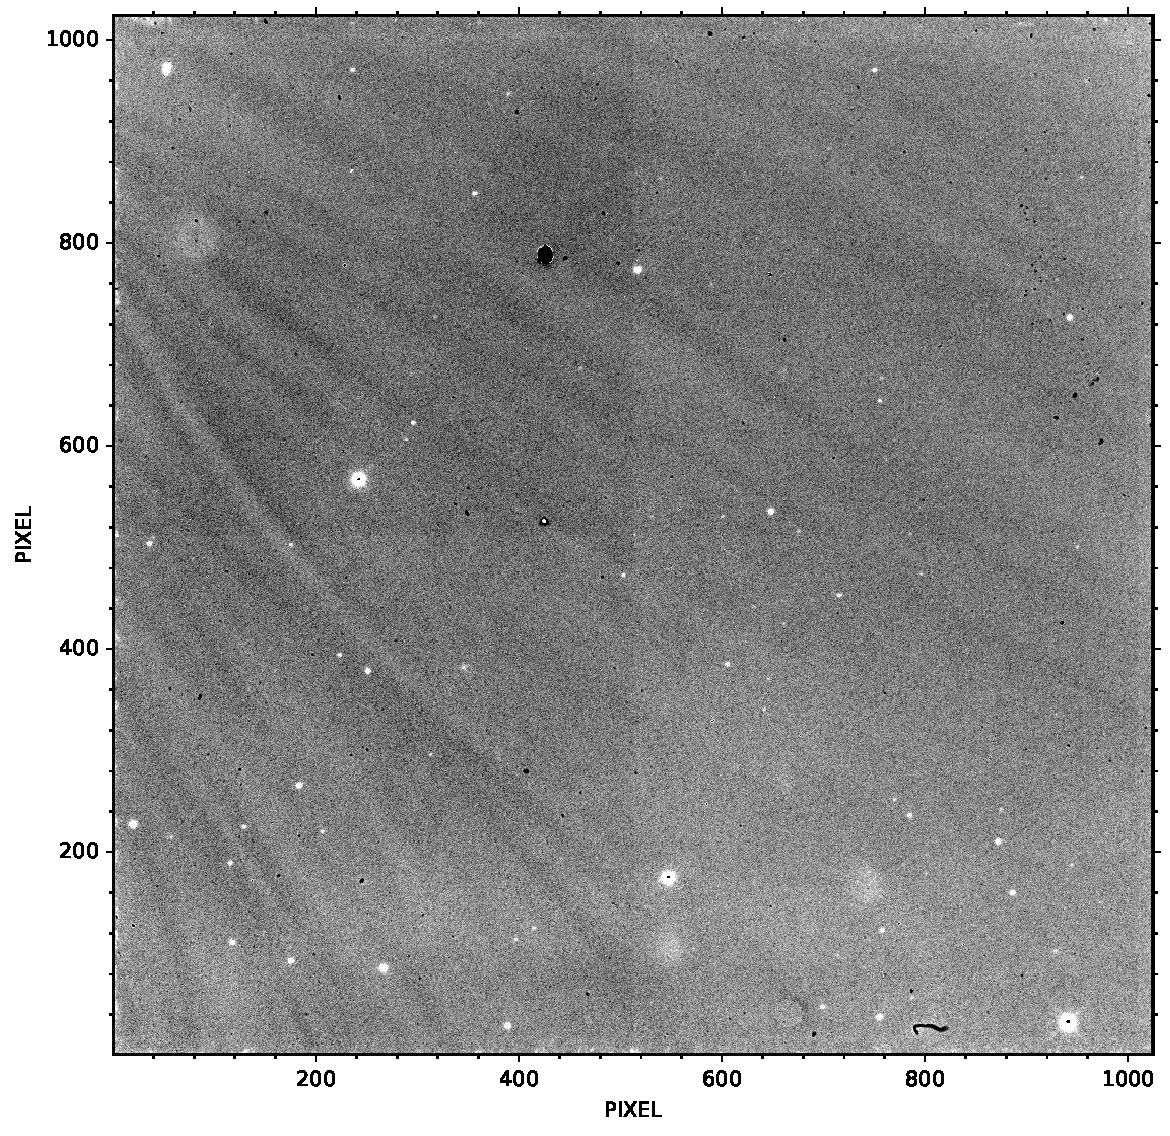
\includegraphics[width=.333\textwidth,clip]{./fig/chap_5/fig_dir_07.pdf}%
	\label{fig:darked_figs_7}%
	}%
  \subfigure[]{%
	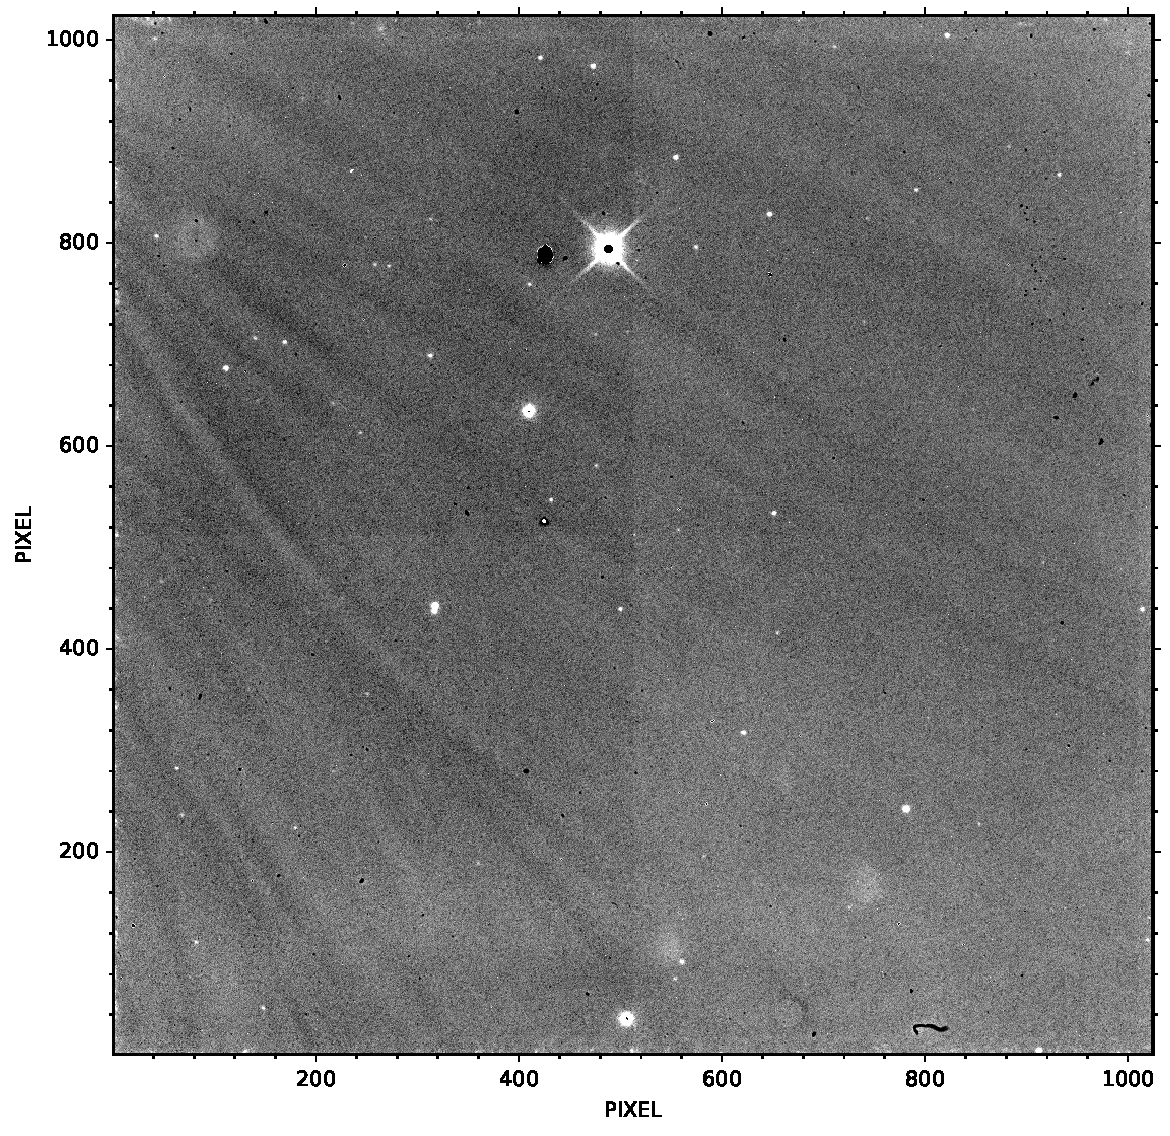
\includegraphics[width=.333\textwidth,clip]{./fig/chap_5/fig_dir_08.pdf}%
	\label{fig:darked_figs_8}%
	}
	\caption{ダーク引き済みの画像}
	\label{fig:darked_figs}
\end{figure}
正直あまり変わった気がしないと思います。これは、十分に冷やされた検出機を使っている場合、熱雑音の成分が目に見えるほど、画像内で支配的になることはないためです。

\subsubsection{フラットフィールディング}
次に、フラットフィールディングの作業に入ります。フラット割りとも言います。現在のデータの状況は
\begin{align*}
  (\text{生データ}) \xrightarrow{\text{ダーク引き}} (感度の違い)\times\left\{ (真の天体信号) + (夜光などの雑音) \right\}
\end{align*}
であって、フラット"割り"というのは、割り算の意味です。感度の違いを補正する画像を作って、割り算をする、ということになります。\par
この「\textbf{フラット}」処理に必要な補正用画像の作成方法には主に次のような方法があります。
\begin{itemize}
  \item ドームフラット
  \begin{itemize}
    \item フラット盤に一様光を反射させる。
    \item 「ライトをつけた状態で撮ったもの」から「ライトを消した状態で撮ったもの」を引けばフラット画像から熱雑音成分が消せる。
    \item 精度悪め。
    \item 天候に左右されない。
    \item 東北大天文の屋上望遠鏡のドームにもフラット盤があるので確認してみて欲しい。
  \end{itemize}
  \item 雲
  \begin{itemize}
    \item 雲の散乱光を観測する。
    \item 雲が一様に光っていると考え、雲の一部を観測する。
    \item ドームフラットよりも精度が良い。
  \end{itemize}
  \item トワイライト
  \begin{itemize}
    \item 夕暮れ時、明け方に撮る。
    \item 太陽が沈む、または昇る時の、明るすぎない時の空を観測する。
  \end{itemize}
\end{itemize}

今回はこの中でも、処理がより簡単なドームフラットを扱うことにします。ドームフラットの工程は次の通りです。
\begin{enumerate}[(1)]
  \item ランプONのドームフラットの平均画像を作成する。
  \item ランプOFFのドームフラットの平均画像を作成する。
  \item ONからOFFを引いた画像を作成する。
  \item この画像を規格化する。
\end{enumerate}

まずはランプONのドームフラットの平均画像を作成します。ダークのときと同様に、画像を結合させれば良いので、
\begin{lstlisting}[caption=ランプONのフラット画像, label=code:flat_light_on]
  # flat
  ## create the flat image
  ### light on
  light_on = np.empty((0, 1024, 1024))
  light_on_fits = sorted(glob.glob('./flat/*.fits'), key=natural_keys)
  for data in light_on_fits:
      light_on_image = fits.getdata(data)
      light_on = np.append(light_on, light_on_image[np.newaxis, :], axis=0)

  median_light_on = np.median(light_on, axis=0)
\end{lstlisting}
とします。

また、ランプOFFの画像ですが、これは作成の仕方からわかるように、これはダーク画像と同等のものなので、今回はダーク画像をランプOFFの画像として扱いましょう。
\begin{lstlisting}[caption=ランプOFFのフラット画像とフラット画像の作成, label=code:flat_light_off]
  ### identify the median dark image as the flat off image
  flat_image = median_light_on - median_dark
\end{lstlisting}

出来上がったflat画像を規格化します。規格化について説明する前に、コード~\ref{code:normalize}を先に示します。
\begin{lstlisting}[caption=フラット画像の規格化,label=code:flatted]
  ## normalize the flat image
  median = np.median(flat_image)
  stddev = np.std(flat_image)
  normalized = np.where(flat_image/median < 0.001, 9999, flat_image/median)
  fits.writeto('./out/flat.fits', normalized, overwrite=True)
\end{lstlisting}
要するに規格化とは、死んだ素子を除外することです。「ONからOFFを引いた画像」で値が極端に小さくなってしまっている素子、具体的には
\begin{verbatim}on_minus_off/median < 0.001\end{verbatim}
であるような素子の情報は、一様に削ぎ落としてしまいたいものです。そこで、flat画像のその素子の値に$9999$という極端な値を入れてしまいます。後でデータをflatで割るのですが、極端に大きな値で割ってしまえば、その素子のデータは極端に0に限りなく近い値となって、無視できるようになるという原理です。ここで作成されたflat画像が図~\ref{fig:flat}です。
\begin{figure}
  \centering
	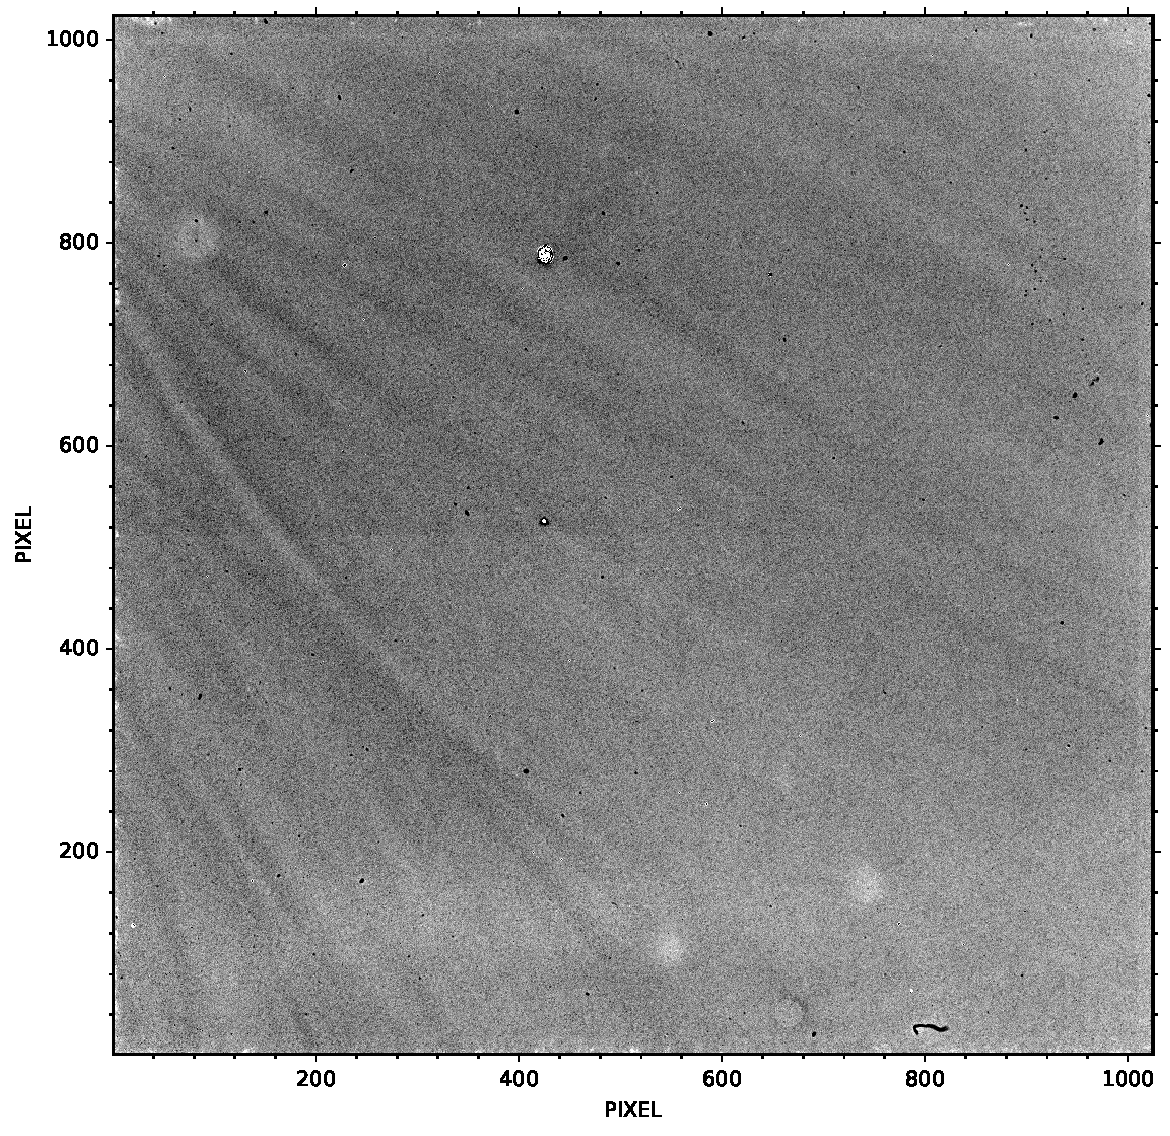
\includegraphics[width=0.6\linewidth]{./fig/chap_5/flat_fits.pdf}
	\caption{フラット画像}
  \label{fig:flat}
\end{figure}

では、作成したflat画像でデータを割る作業に移ります。割るという作業も単純な演算で、
\begin{lstlisting}[caption=フラット割り,label=code:flatting]
  ## flat the images
  dir_images = sorted(glob.glob('./out/dir_*.fits'), key=natural_keys)
  for i, data in enumerate(dir_images):
      img = fits.getdata(data)
      flat = img/normalized
      file_name = 'fdir_' + str('{:02d}'.format(i)) + '.fits'
      fits.writeto('./out/' + file_name, flat, overwrite=True)
\end{lstlisting}
となります。ここまでの作業が完了したfdir画像を表示してみると図~\ref{fig:flatted}のようになります。よくみると画像に模様のようなものがうっすらと入っています。これは次のスカイ引きの処理で取り除くものなので、ここでは問題ありません。
\begin{figure}
	\centering
	\subfigure[]{%
	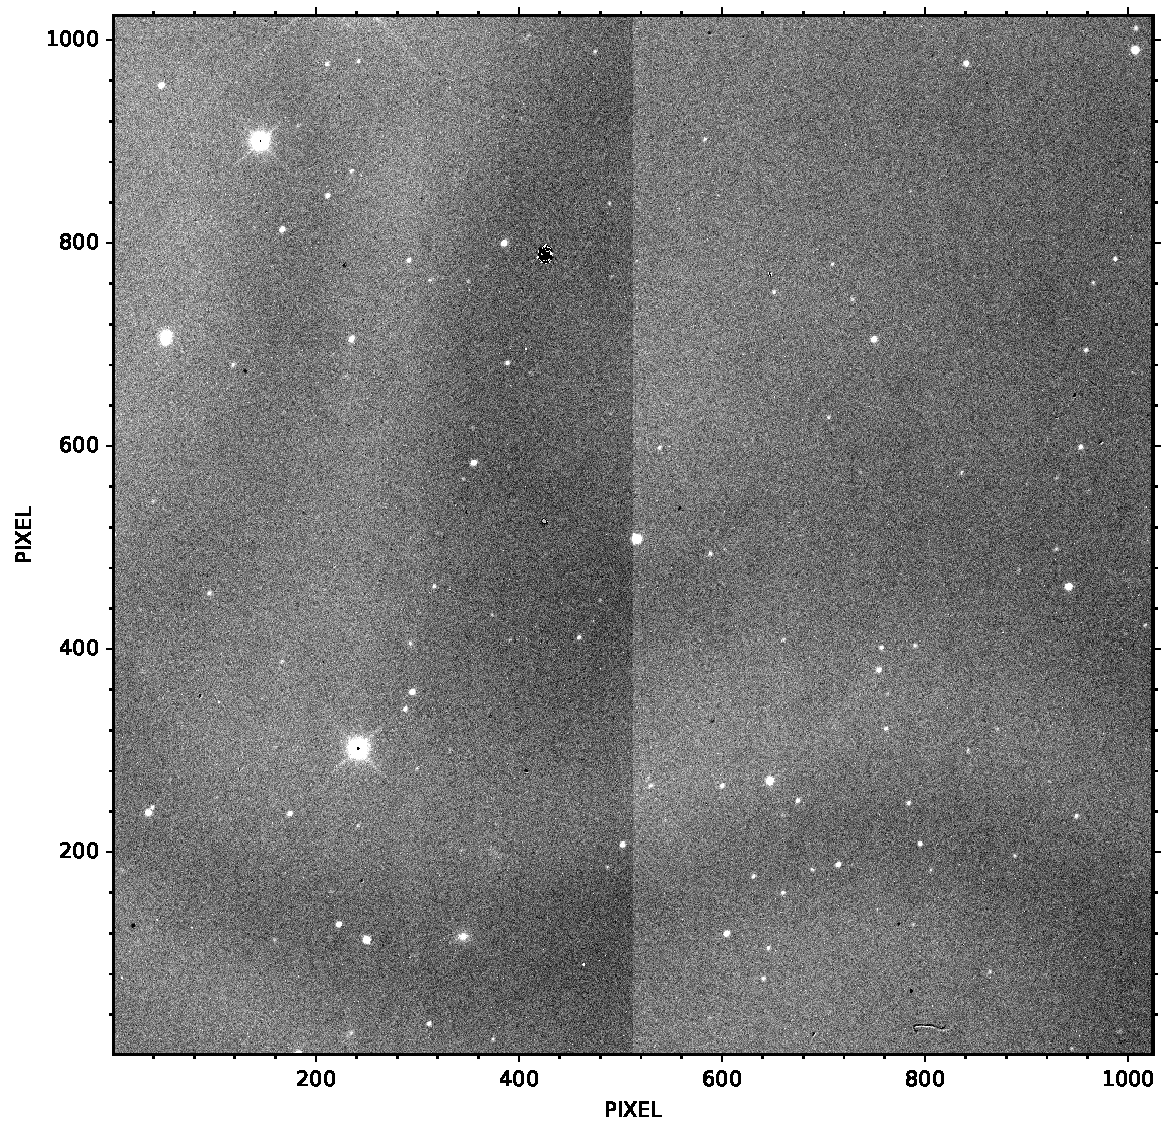
\includegraphics[width=.333\textwidth,clip]{./fig/chap_5/fig_fdir_00.pdf}%
	\label{fig:flatted_figs_0}%
	}%
	\subfigure[]{%
	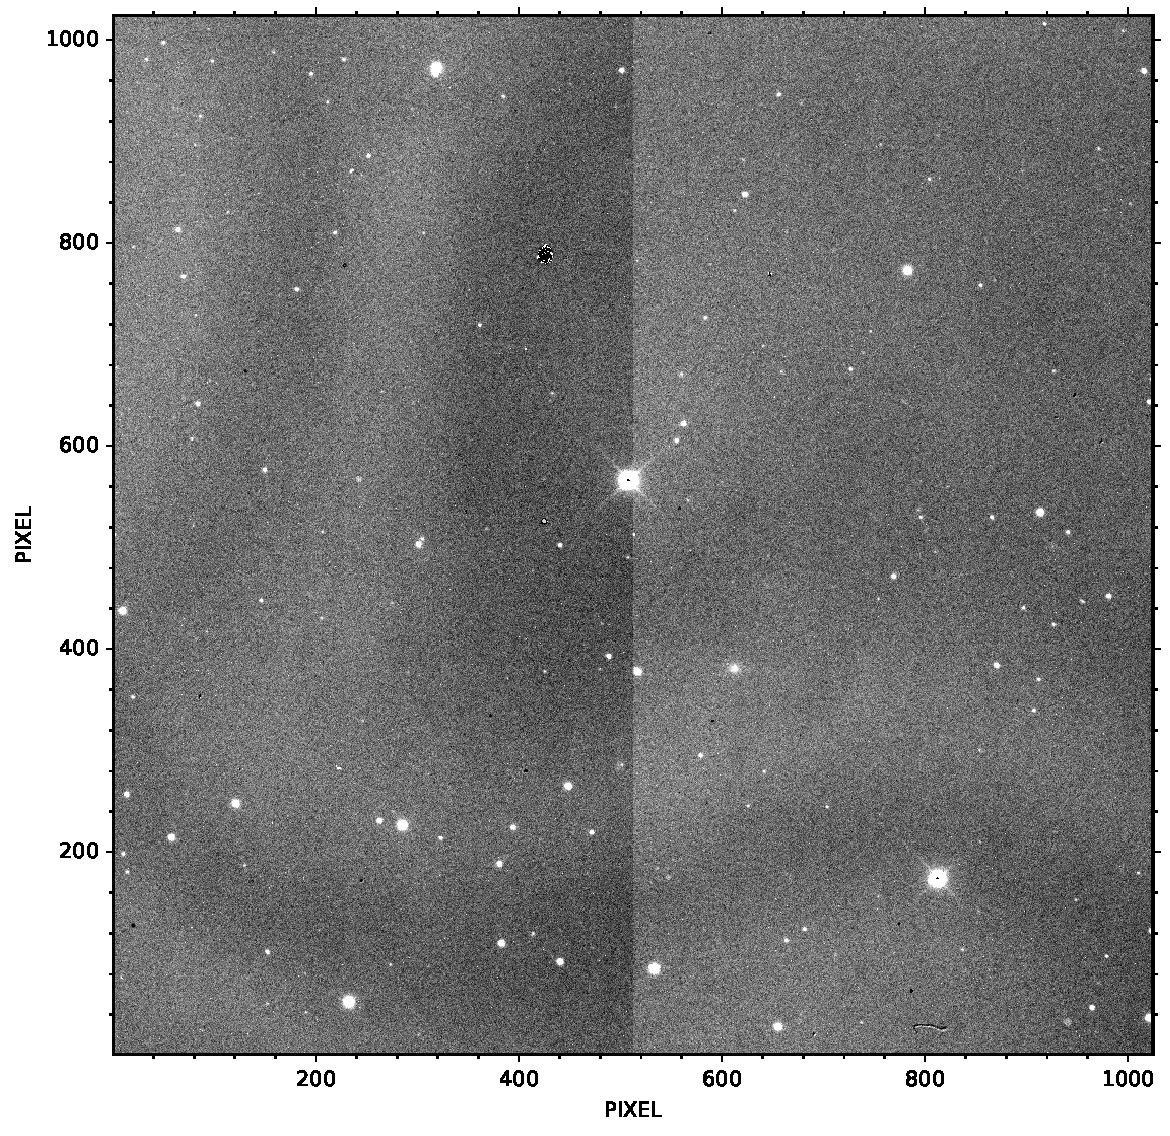
\includegraphics[width=.333\textwidth,clip]{./fig/chap_5/fig_fdir_01.pdf}%
	\label{fig:flatted_figs_1}%
	}%
  \subfigure[]{%
	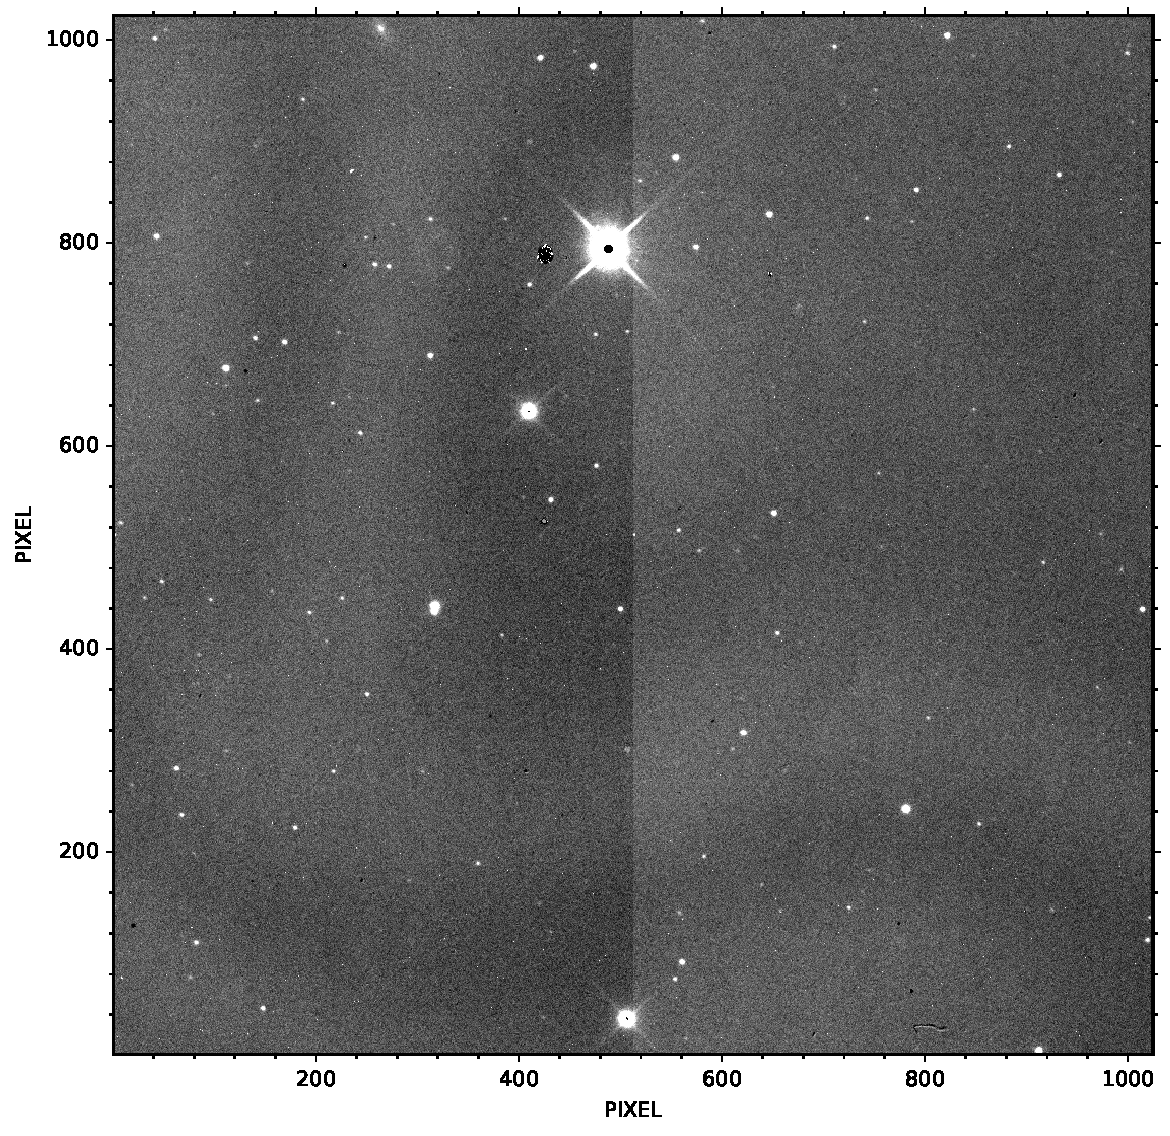
\includegraphics[width=.333\textwidth,clip]{./fig/chap_5/fig_fdir_02.pdf}%
	\label{fig:flatted_figs_2}%
	}
  \subfigure[]{%
	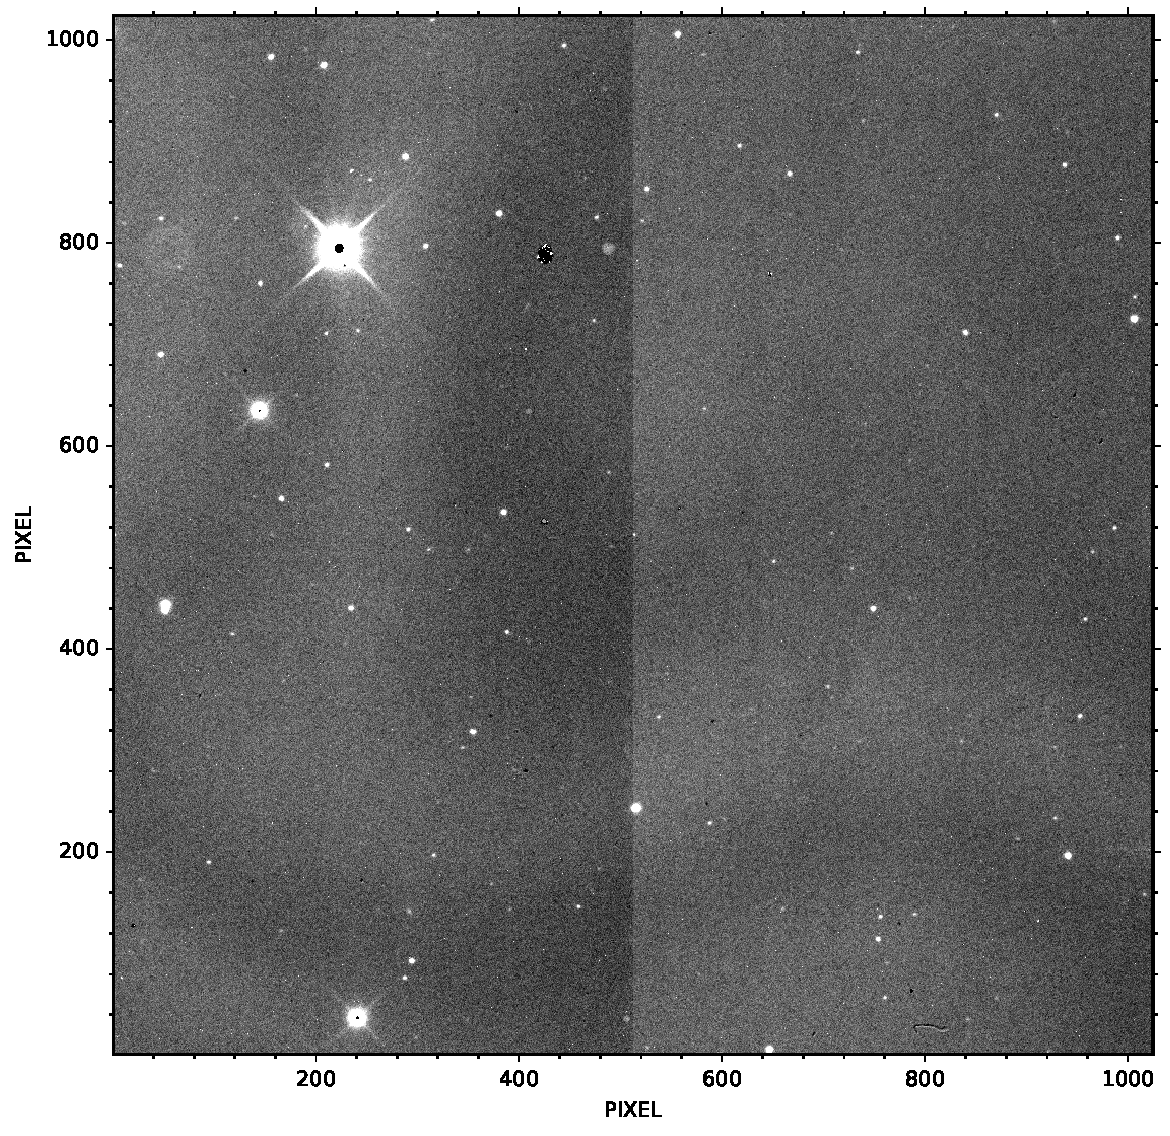
\includegraphics[width=.333\textwidth,clip]{./fig/chap_5/fig_fdir_03.pdf}%
	\label{fig:flatted_figs_3}%
	}%
	\subfigure[]{%
	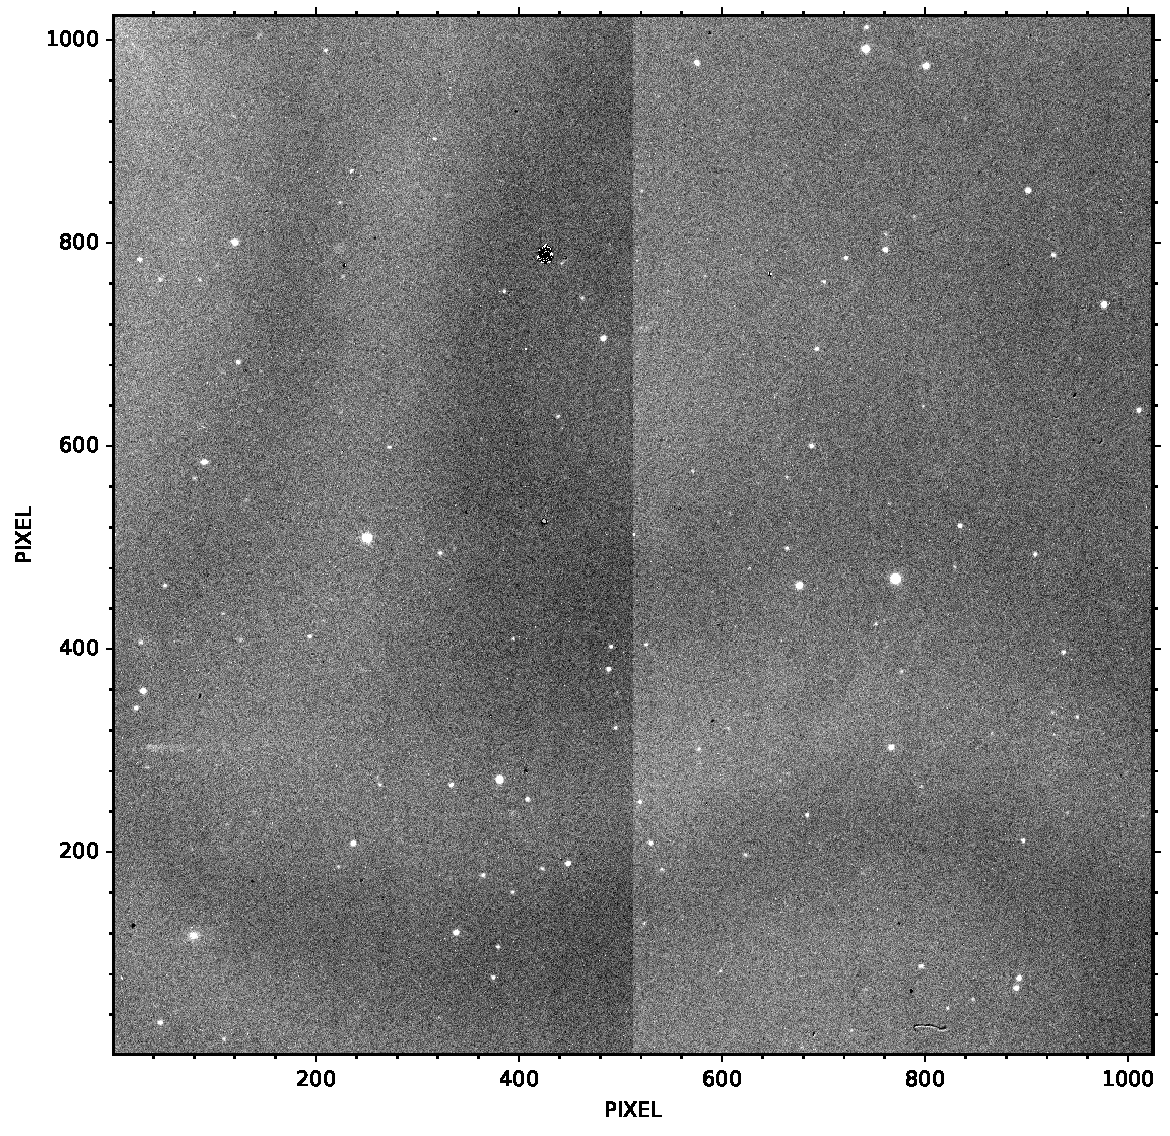
\includegraphics[width=.333\textwidth,clip]{./fig/chap_5/fig_fdir_04.pdf}%
	\label{fig:flatted_figs_4}%
	}%
  \subfigure[]{%
	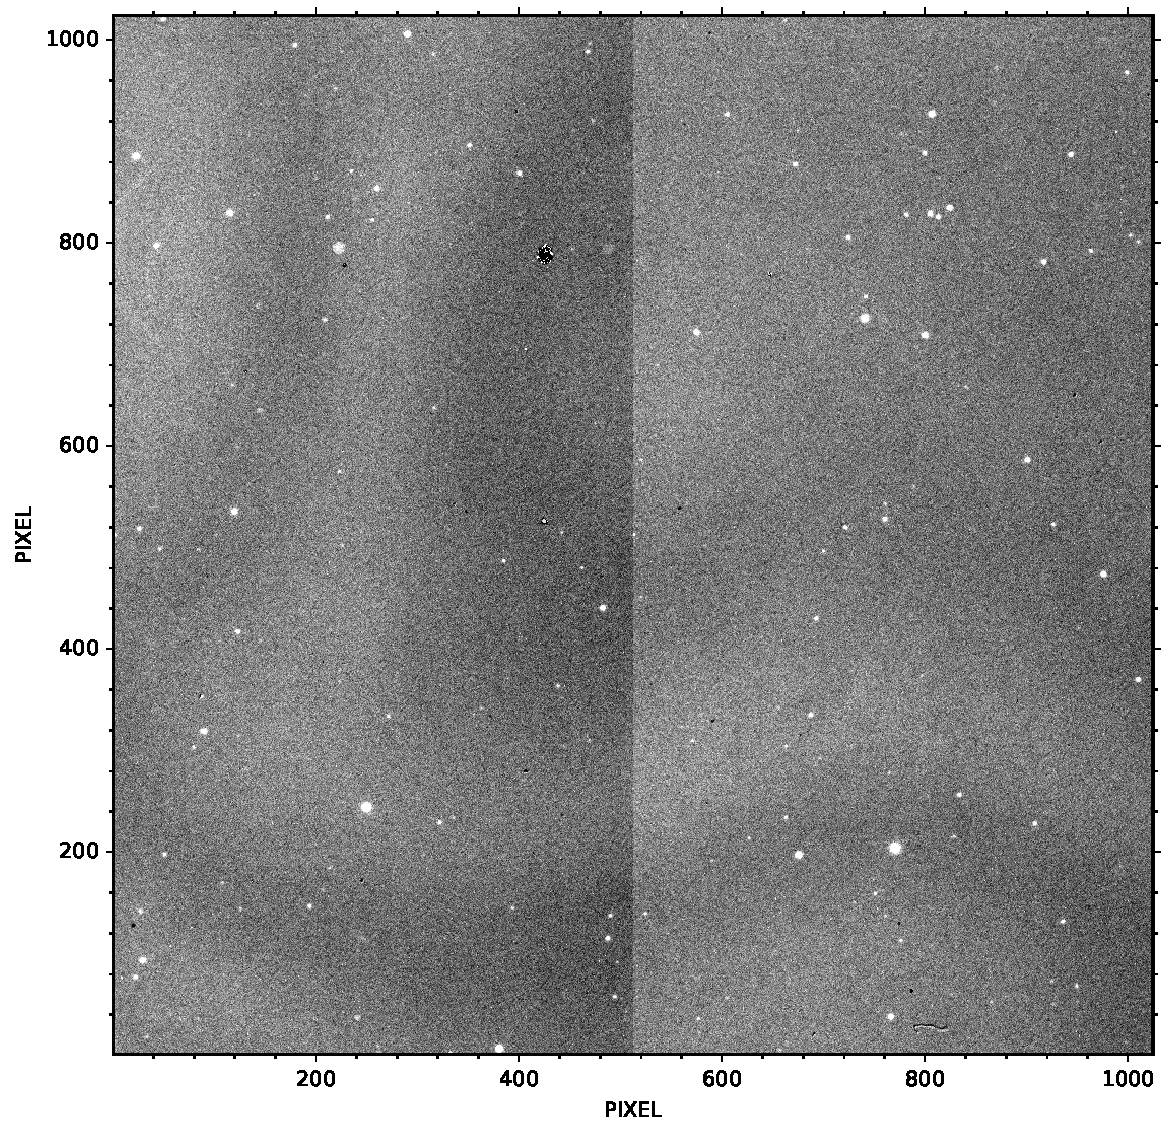
\includegraphics[width=.333\textwidth,clip]{./fig/chap_5/fig_fdir_05.pdf}%
	\label{fig:flatted_figs_5}%
	}
  \subfigure[]{%
	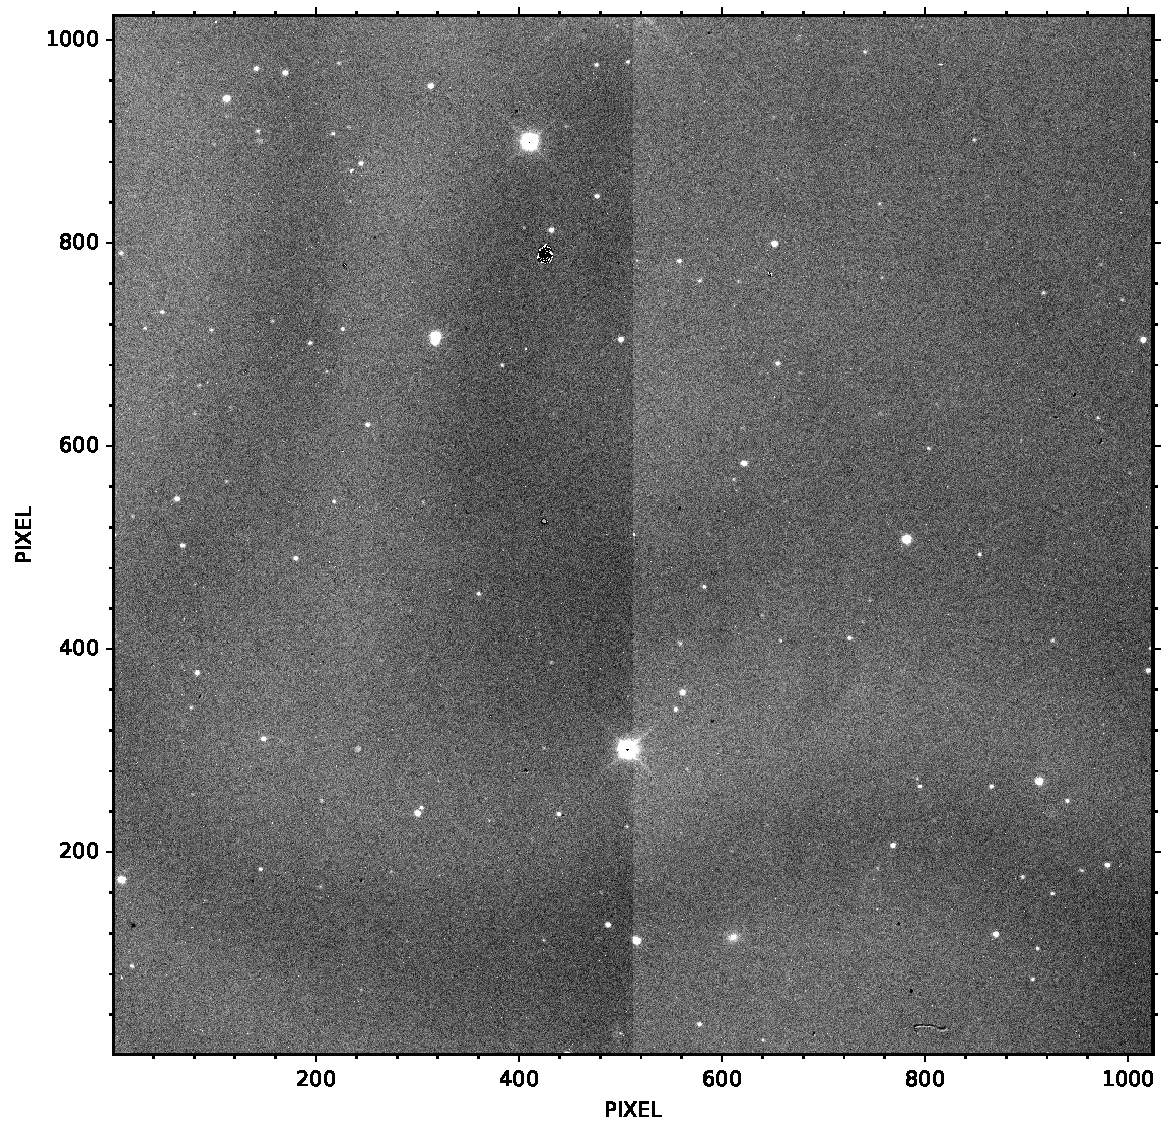
\includegraphics[width=.333\textwidth,clip]{./fig/chap_5/fig_fdir_06.pdf}%
	\label{fig:flatted_figs_6}%
	}%
	\subfigure[]{%
	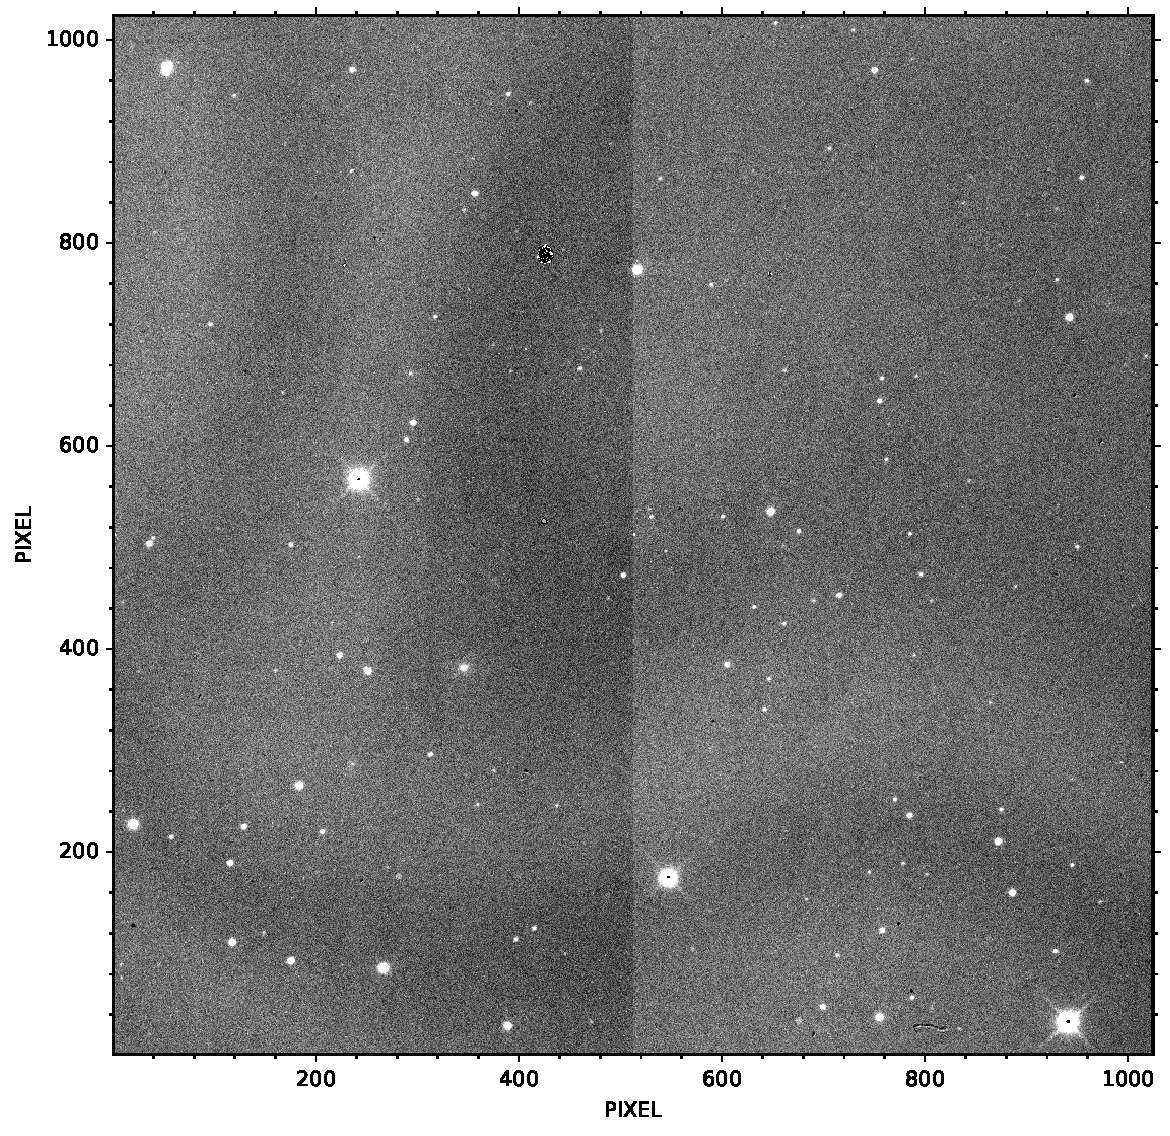
\includegraphics[width=.333\textwidth,clip]{./fig/chap_5/fig_fdir_07.pdf}%
	\label{fig:flatted_figs_7}%
	}%
  \subfigure[]{%
	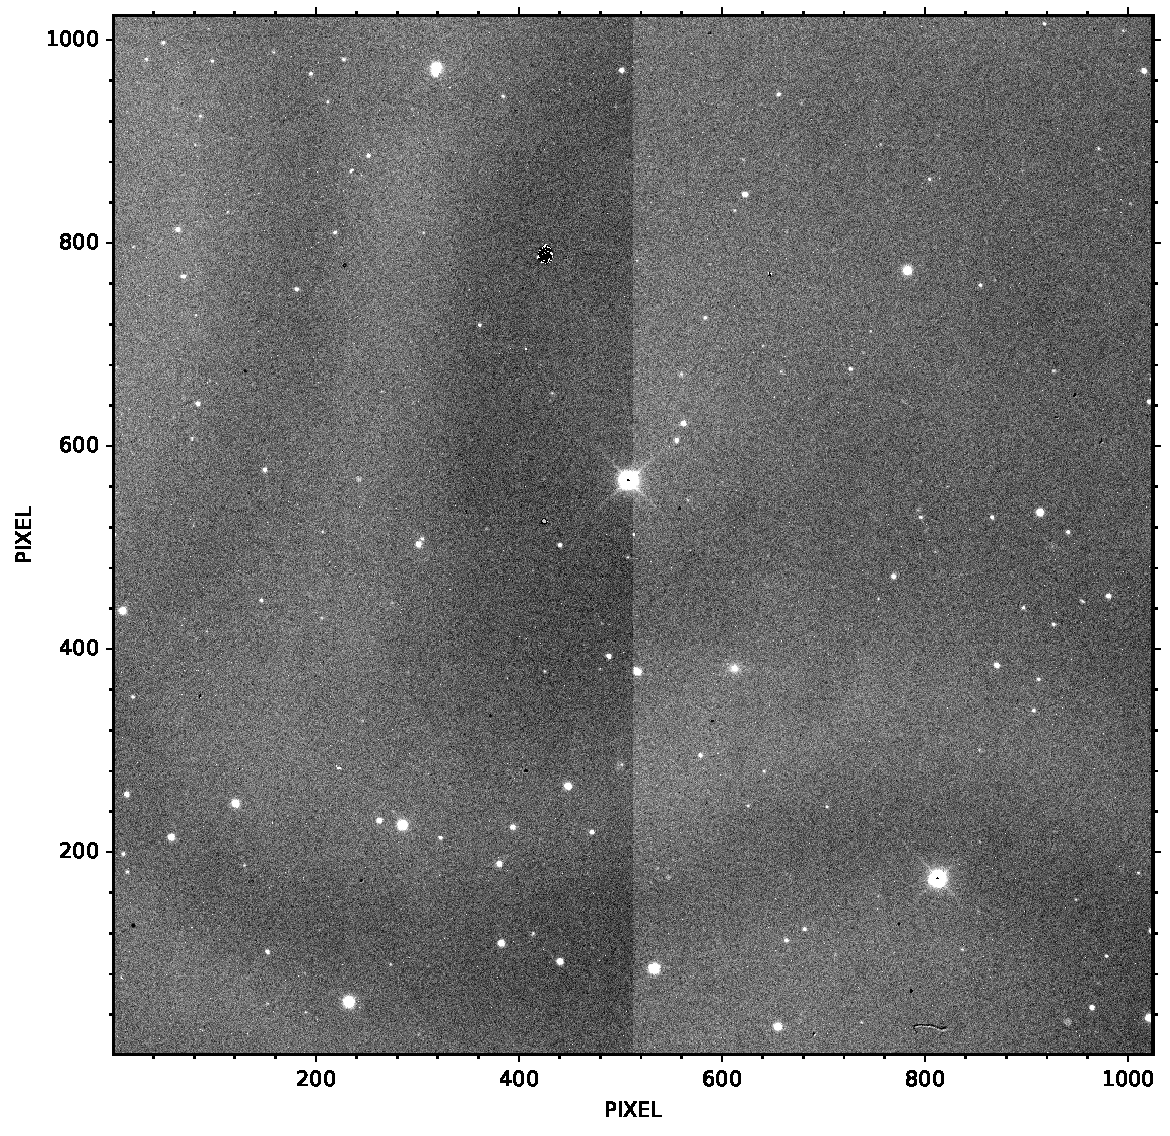
\includegraphics[width=.333\textwidth,clip]{./fig/chap_5/fig_fdir_08.pdf}%
	\label{fig:flatted_figs_8}%
	}
	\caption{フラットフィールディング済みの画像}
	\label{fig:flatted}
\end{figure}

この作業によって素子ごとの感度の違いが補正され、
\begin{align*}
  (\text{生データ}) &\xrightarrow{\text{ダーク引き}} (感度の違い)\times\left\{ (真の天体信号) + (夜光などの雑音) \right\} \\
  &\xrightarrow{\text{フラットフィールディング}} \left\{ (真の天体信号) + (夜光などの雑音) \right\}
\end{align*}
となりました。

\subsubsection{スカイ引き}
1次処理の最後はスカイ引きの処理に入ります。スカイ画像は、感度補正が終わった全ての画像を重ねて、その中央値をとれば作成できます。
\begin{lstlisting}[caption=スカイ画像の作成,label=code:sky_image]
  # sky
  ## create the sky image
  sky_images = np.empty((0, 1024, 1024))
  fdir_images = sorted(glob.glob('./out/fdir_*.fits'), key=natural_keys)
  for data in fdir_images:
      sky = fits.getdata(data)
      sky_images = np.append(sky_images, sky[np.newaxis, :], axis=0)
  
  median_sky = np.median(sky_images, axis=0)
  fits.writeto('./out/sky.fits', median_sky, overwrite=True)
\end{lstlisting}

できたスカイ画像が図~\ref{fig:sky_image}のようになります。星が消えて、模様のようなものだけ見えています。
\begin{figure}
  \centering
  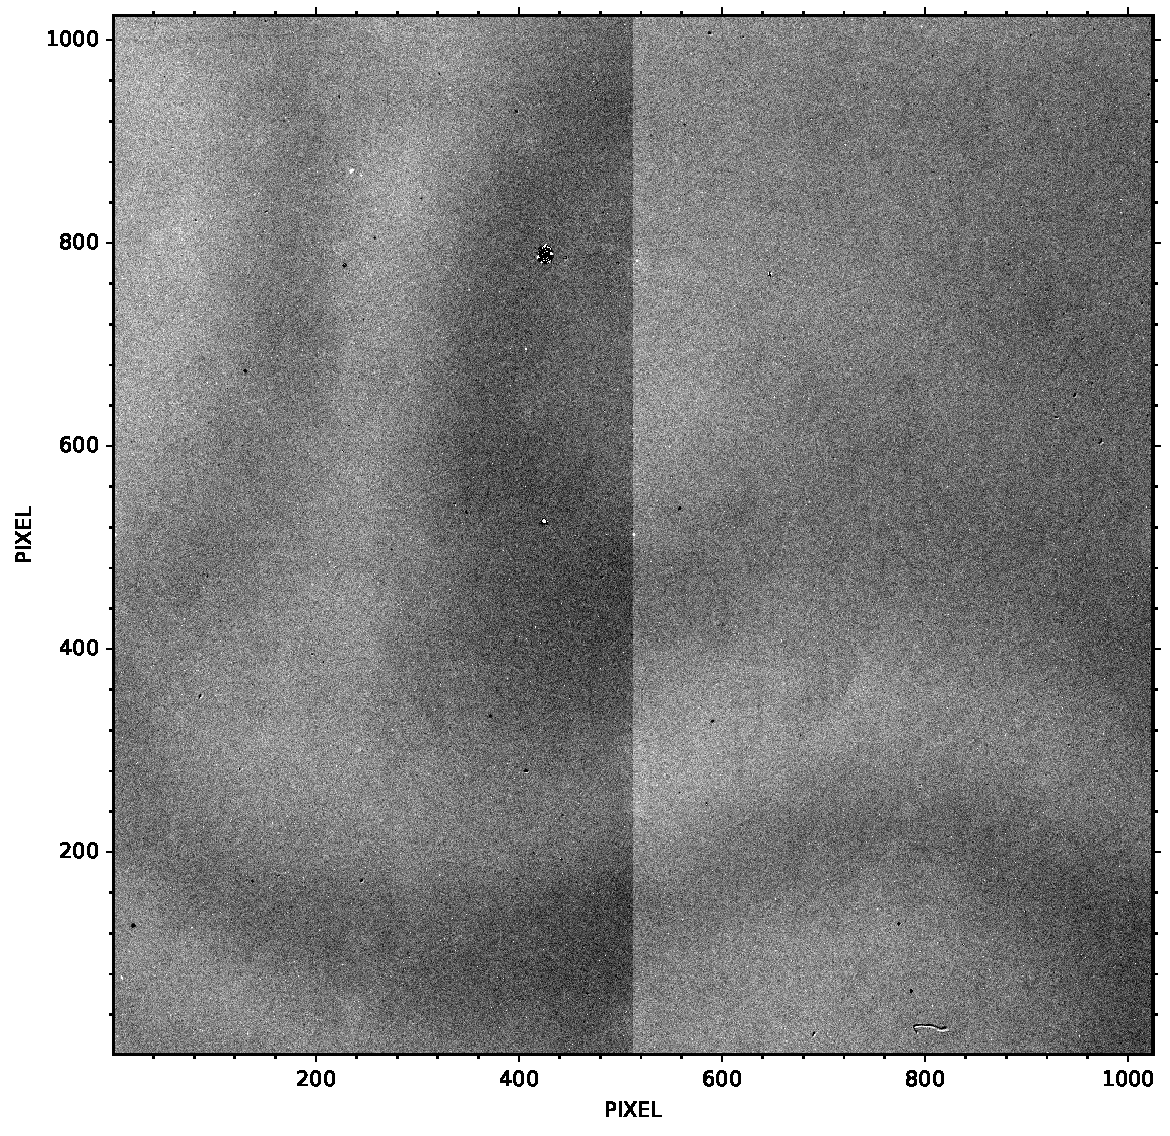
\includegraphics[width=0.6\linewidth]{./fig/chap_5/sky_fits.pdf}
  \caption{スカイ画像}
  \label{fig:sky_image}
\end{figure}
ここではダーク引きと同様に単純に引くだけなので、
\begin{lstlisting}[caption=スカイ引き,label=code:subtract_sky]
  ## subtract the sky data from fdir data
  for i, data in enumerate(fdir_images):
      img = fits.getdata(data)
      sub_sky = img - median_sky
      file_name = 'sfdir_' + str('{:02d}'.format(i)) + '.fits'
      fits.writeto('./out/' + file_name, sub_sky, overwrite=True)
\end{lstlisting}
となります。ここでも例によって、「s」をつけてスカイ引き済みという意味にしています。
できた画像を表示させてみます。コード的には次のようにします。
\begin{lstlisting}[caption=作成した画像の表示,label=code:kansei]
  sfdir_images = sorted(glob.glob('./out/sfdir_*.fits'), key=natural_keys)
  for i,data in enumerate(sfdir_images):
      img = fits.open(data)
      pic = aplpy.FITSFigure(img)
      pic.show_grayscale()
      img_name = 'fig_' + str('{:02d}'.format(i)) + '.pdf'
      pic.save('./fig/' + img_name)
\end{lstlisting}

これで表示される画像は図~\ref{fig:skyed}です。
\begin{figure}
	\centering
	\subfigure[]{%
	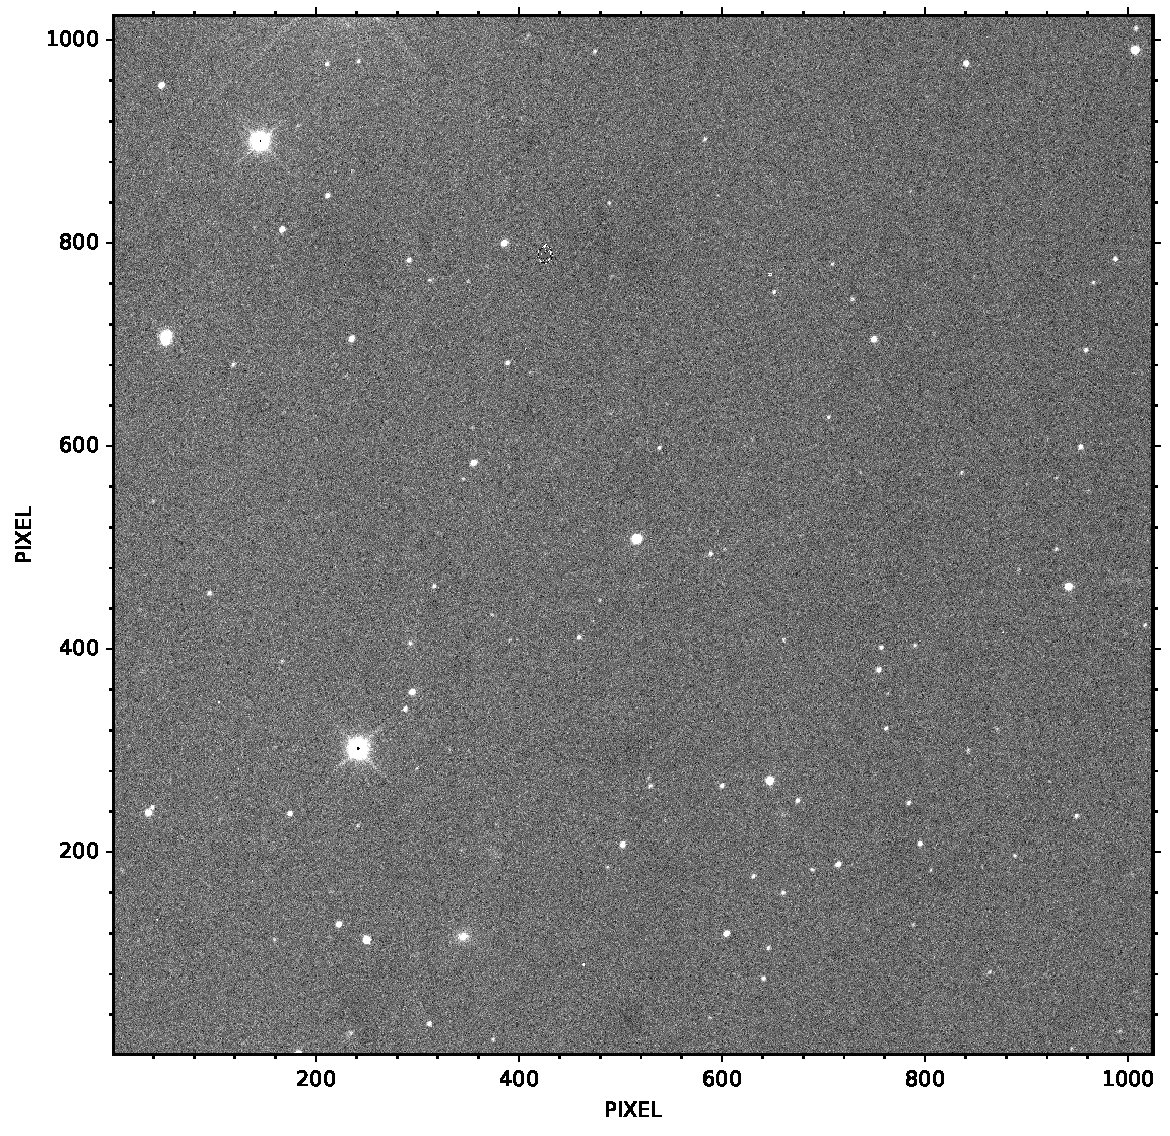
\includegraphics[width=.333\textwidth,clip]{./fig/chap_5/fig_00.pdf}%
	\label{fig:skyed_figs_0}%
	}%
	\subfigure[]{%
	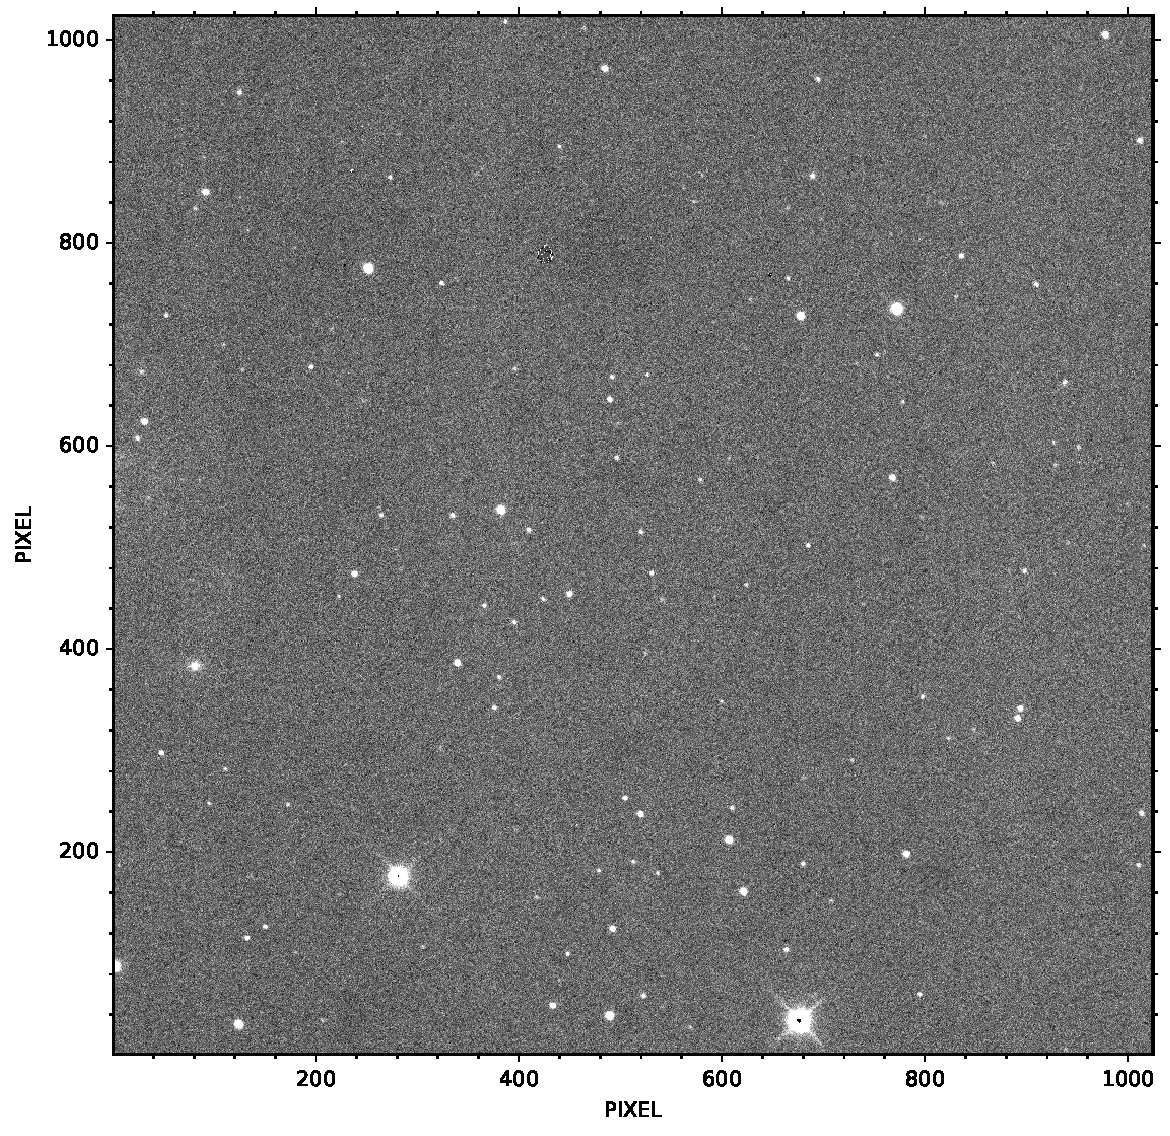
\includegraphics[width=.333\textwidth,clip]{./fig/chap_5/fig_01.pdf}%
	\label{fig:skyed_figs_1}%
	}%
  \subfigure[]{%
	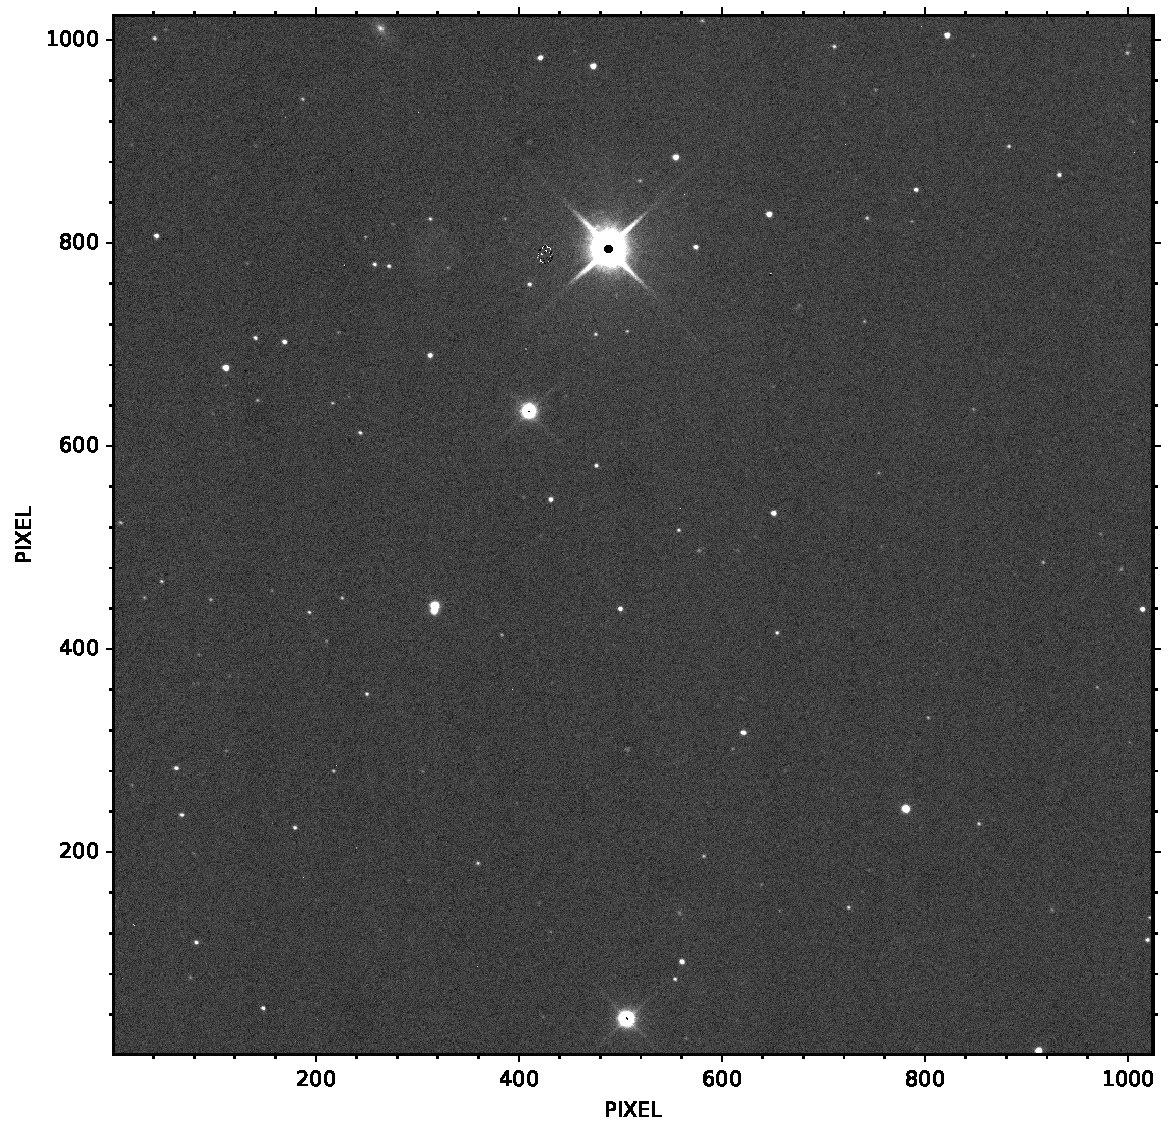
\includegraphics[width=.333\textwidth,clip]{./fig/chap_5/fig_02.pdf}%
	\label{fig:skyed_figs_2}%
	}
  \subfigure[]{%
	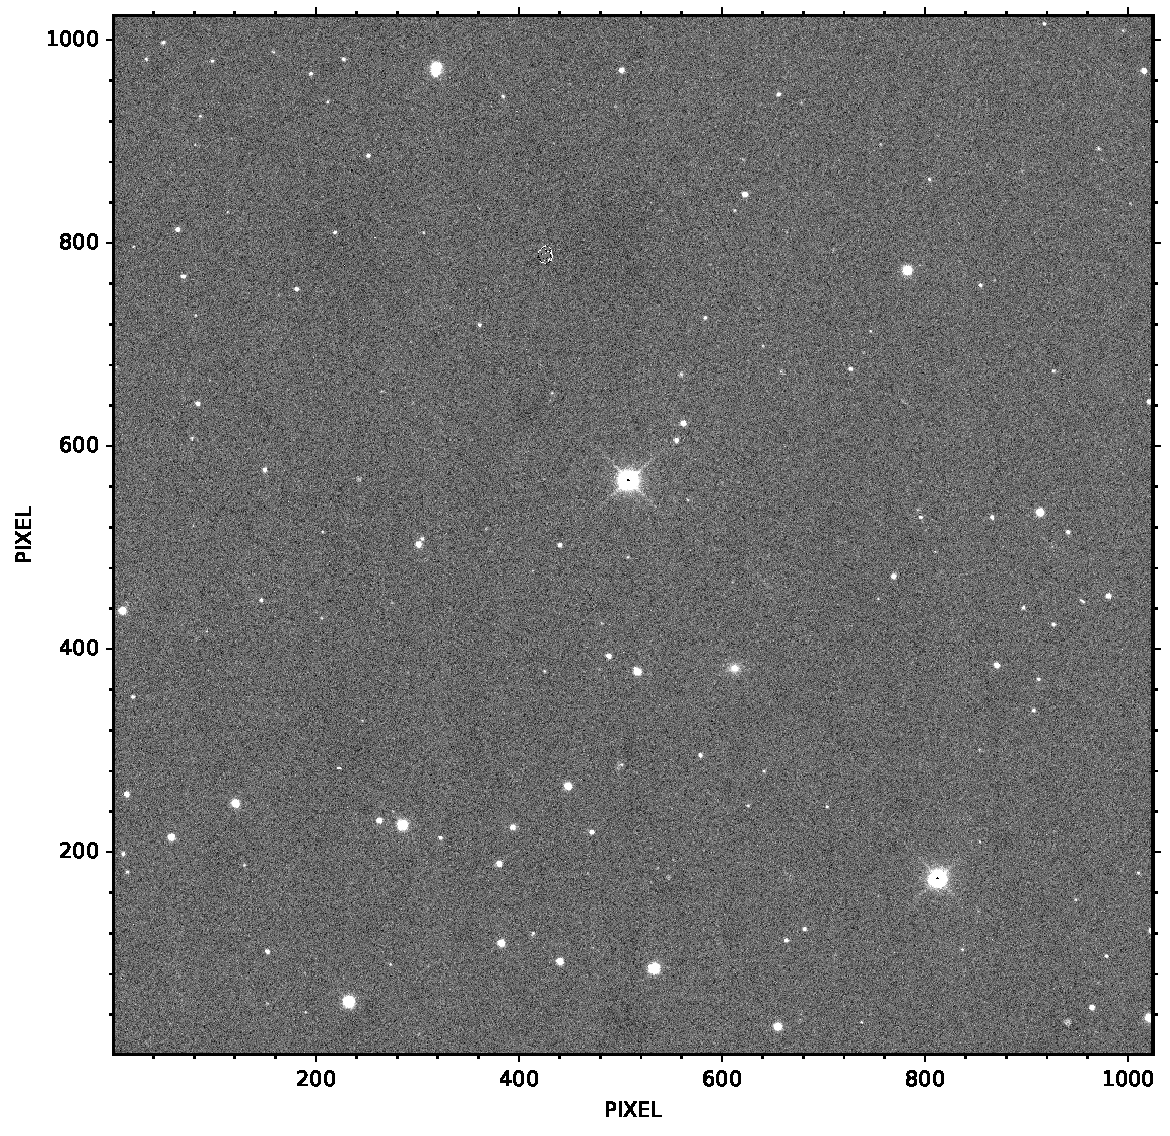
\includegraphics[width=.333\textwidth,clip]{./fig/chap_5/fig_03.pdf}%
	\label{fig:skyed_figs_3}%
	}%
	\subfigure[]{%
	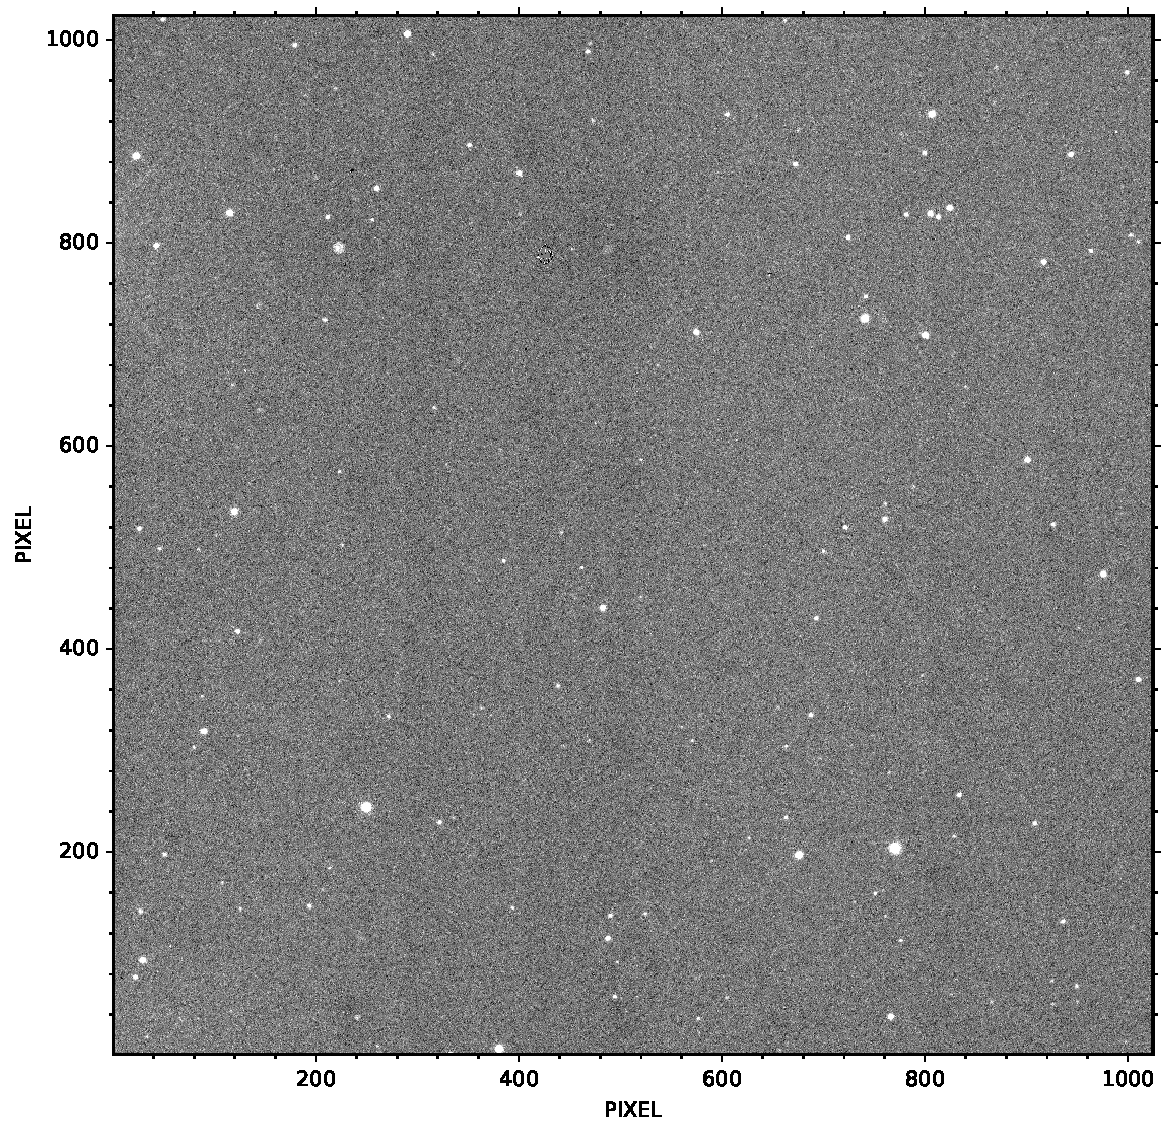
\includegraphics[width=.333\textwidth,clip]{./fig/chap_5/fig_04.pdf}%
	\label{fig:skyed_figs_4}%
	}%
  \subfigure[]{%
	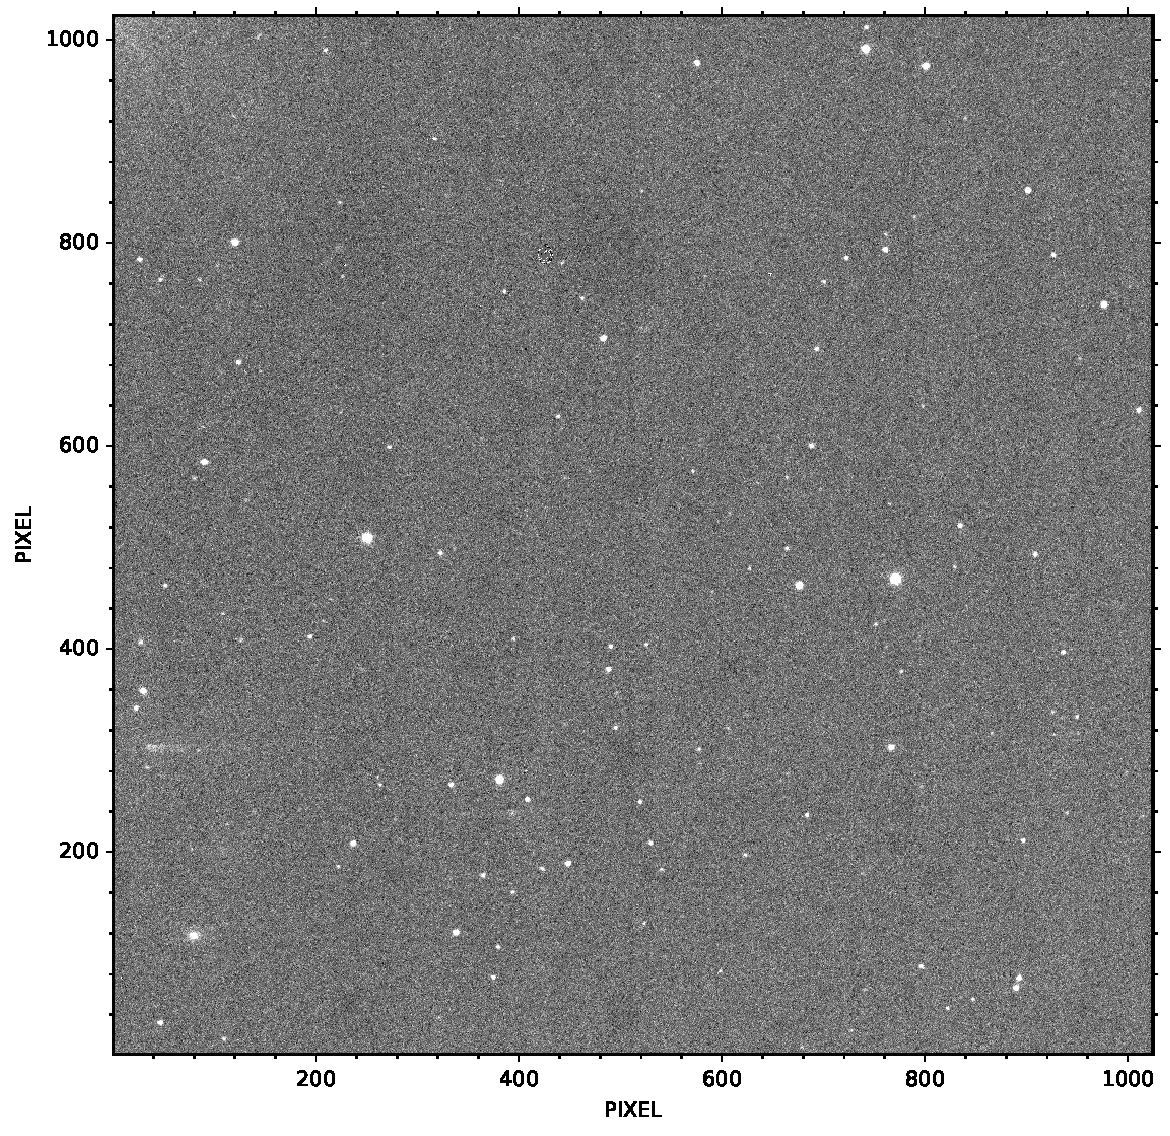
\includegraphics[width=.333\textwidth,clip]{./fig/chap_5/fig_05.pdf}%
	\label{fig:skyed_figs_5}%
	}
  \subfigure[]{%
	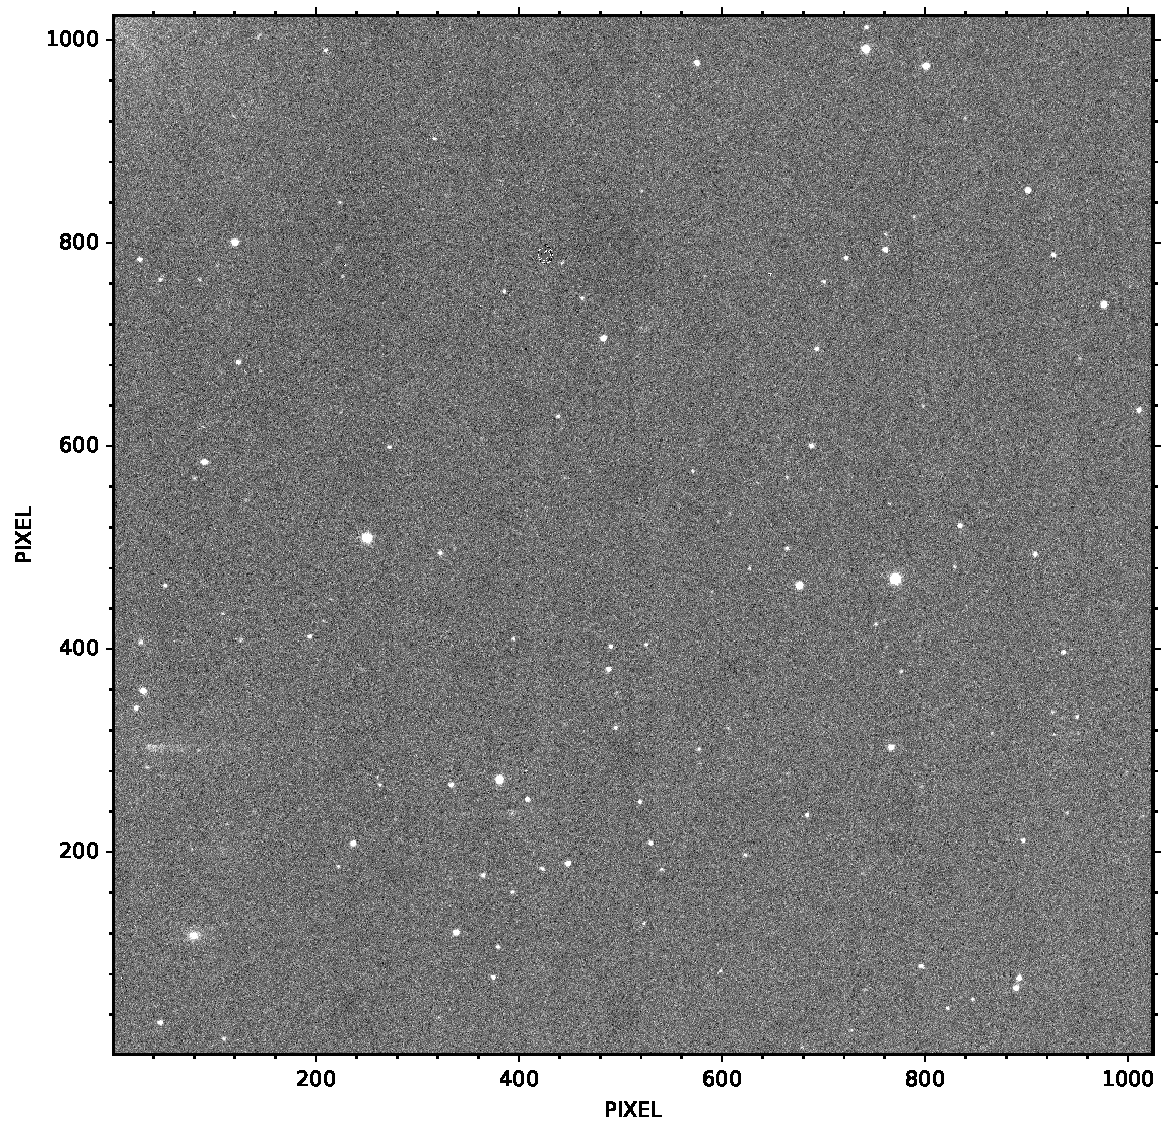
\includegraphics[width=.333\textwidth,clip]{./fig/chap_5/fig_06.pdf}%
	\label{fig:skyed_figs_6}%
	}%
	\subfigure[]{%
	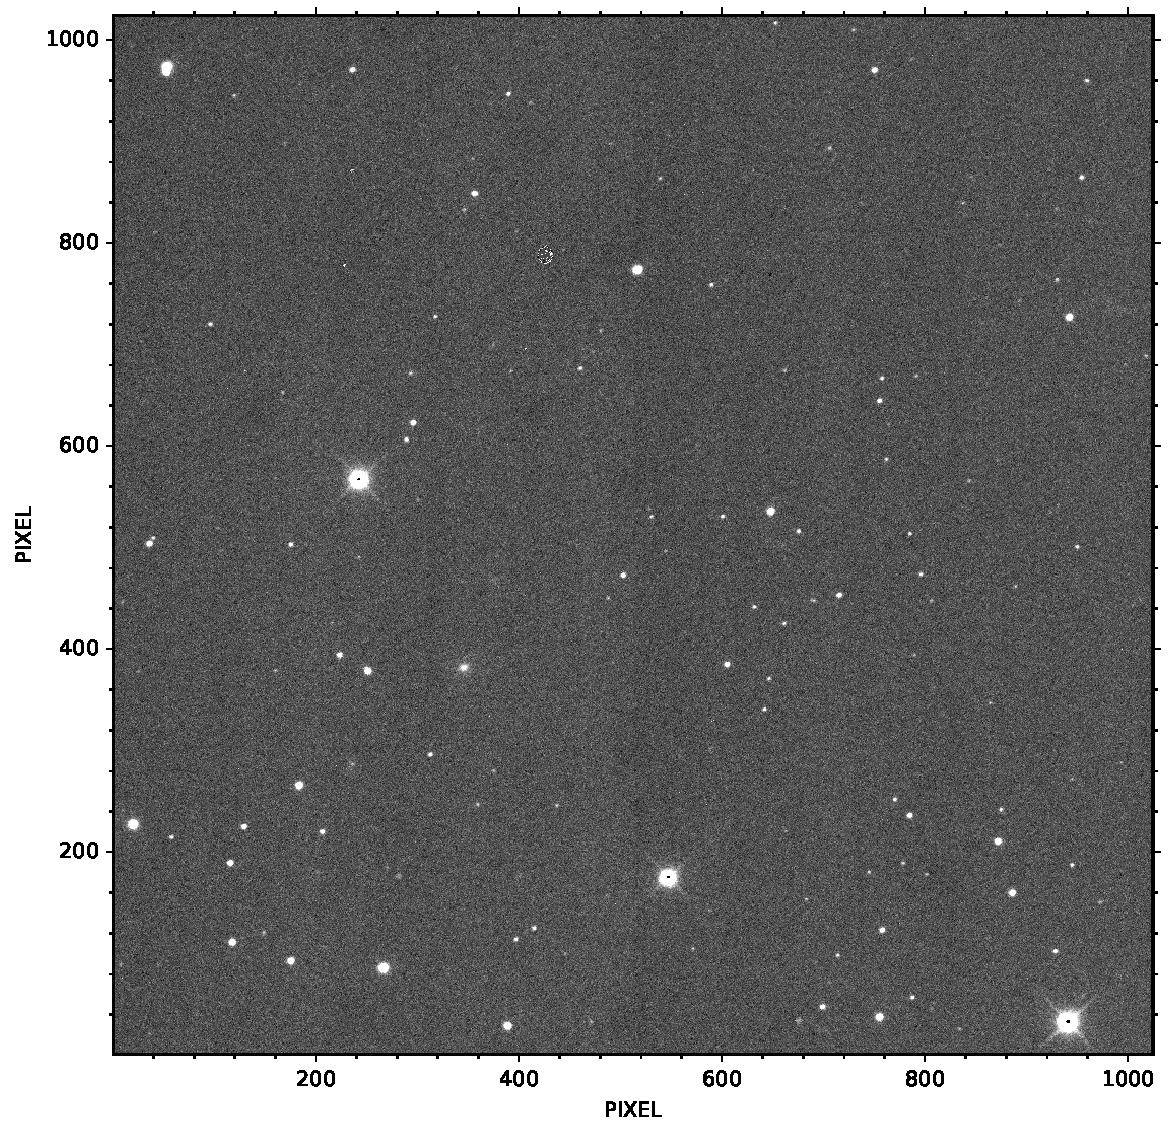
\includegraphics[width=.333\textwidth,clip]{./fig/chap_5/fig_07.pdf}%
	\label{fig:skyed_figs_7}%
	}%
  \subfigure[]{%
	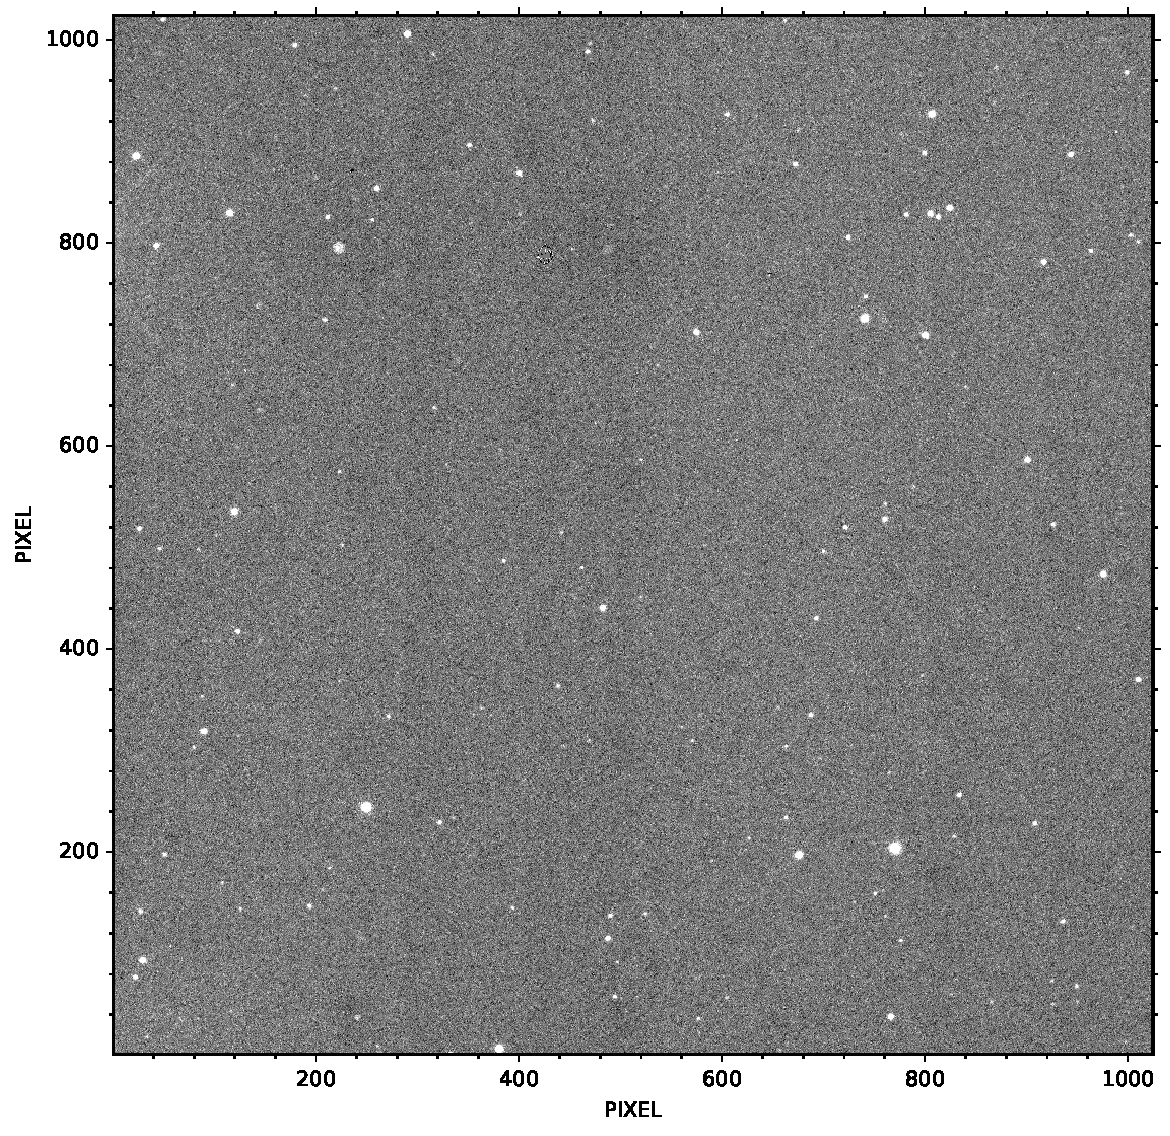
\includegraphics[width=.333\textwidth,clip]{./fig/chap_5/fig_08.pdf}%
	\label{fig:skyed_figs_8}%
	}
	\caption{sky引きまでの処理が終わった画像}
	\label{fig:skyed}
\end{figure}
変な模様が消えたので、綺麗な画像になっているのがわかります。これで1次処理は終わりです。スカイ引きによって
\begin{align*}
  (\text{生データ}) &\xrightarrow{\text{ダーク引き}} (感度の違い)\times\left\{ (真の天体信号) + (夜光などの雑音) \right\} \\
  &\xrightarrow{\text{フラットフィールディング}} \left\{ (真の天体信号) + (夜光などの雑音) \right\} \\
  &\xrightarrow{\text{スカイ引き}} (真の天体信号)
\end{align*}
となりました。

\subsubsection{1次処理のまとめ}
ここまでで行った1次処理の解析コードをまとめます。実行的には、\texttt{raw}に観測の生データ、\texttt{dark}にダークのデータ、\texttt{flat}にフラット画像を作る際のライトオンのデータを入れてしまえば、以下のコードを走らせるだけで1次処理が完了します\footnote{ただし、2021年度のもし天のように、データ自体に不具合が生じている場合、例えば生データ取得時とフラットデータ取得時でCCDの角度が異なっているなどした時には、画像を回転させるなどの処置が必要になります。当日そのような事態におちいると非常に焦るので、あらかじめどのような不具合が想定されるかどうか考えておくとよいかもしれません。}。
\begin{lstlisting}[caption=1次処理のまとめ,label=code:itizisyori]
  import os
  import re
  import numpy as np
  import astropy.io.fits as fits
  import glob
  import matplotlib.pyplot as plt
  import aplpy

  # create a directory if that directory does not exist
  def my_makedirs(path):
      if not os.path.isdir(path):
          os.makedirs(path)
  my_makedirs('./out')


  # functions for the function "sorted()"
  def atoi(text):
      return int(text) if text.isdigit() else text
  def natural_keys(text):
      return [ atoi(c) for c in re.split(r'(\d+)', text) ]


  # dark
  ## merge the dark images
  dark_images = np.empty((0, 1024, 1024)) 
  dark_fits = sorted(glob.glob('./dark/*.fits'), key=natural_keys)
  for data in dark_fits:
      dark = fits.getdata(data)
      dark_images = np.append(dark_images, dark[np.newaxis, :], axis=0)

  median_dark = np.median(dark_images, axis=0)
  fits.writeto('./out/dark.fits', median_dark, overwrite=True)

  ## subtract the dark data from raw data
  dark = fits.getdata('./out/dark.fits')
  raw_fits = sorted(glob.glob('./raw/*.fits'), key=natural_keys)
  for i,data in enumerate(raw_fits):
      raw_image = fits.getdata(data)
      sub_dark = raw_image - dark
      file_name = 'dir_' + str('{:02d}'.format(i)) + '.fits'
      fits.writeto('./out/' + file_name, sub_dark, overwrite=True)


  # flat
  ## create the flat images
  ### light on
  light_on = np.empty((0, 1024, 1024))
  light_on_fits = sorted(glob.glob('./flat/*.fits'), key=natural_keys)
  for data in light_on_fits:
      light_on_image = fits.getdata(data)
      light_on = np.append(light_on, light_on_image[np.newaxis, :], axis=0)

  median_light_on = np.median(light_on, axis=0)

  ### identify the median dark image as the flat off image
  flat_image = median_light_on - median_dark

  ## normalize the flat image
  median = np.median(flat_image)
  stddev = np.std(flat_image)
  normalized = np.where(flat_image/median < 0.001, 9999, flat_image/median)
  fits.writeto('./out/flat.fits', normalized, overwrite=True)

  ## flat the images
  dir_images = sorted(glob.glob('./out/dir_*.fits'), key=natural_keys)
  print(dir_images)
  for i, data in enumerate(dir_images):
      img = fits.getdata(data)
      flat = img/normalized
      file_name = 'fdir_' + str('{:02d}'.format(i)) + '.fits'
      fits.writeto('./out/' + file_name, flat, overwrite=True)


  # sky
  ## create the sky image
  sky_images = np.empty((0, 1024, 1024))
  fdir_images = sorted(glob.glob('./out/fdir_*.fits'), key=natural_keys)
  for data in fdir_images:
      sky = fits.getdata(data)
      sky_images = np.append(sky_images, sky[np.newaxis, :], axis=0)

  median_sky = np.median(sky_images, axis=0)
  fits.writeto('./out/sky.fits', median_sky, overwrite=True)

  ## subtract the sky data from fdir data
  for i, data in enumerate(fdir_images):
      img = fits.getdata(data)
      sub_sky = img - median_sky
      file_name = 'sfdir_' + str('{:02d}'.format(i)) + '.fits'
      fits.writeto('./out/' + file_name, sub_sky, overwrite=True)

  # visualize the image
  my_makedirs('./fig')
  sfdir_images = sorted(glob.glob('./out/sfdir_*.fits'), key=natural_keys)
  for i,data in enumerate(sfdir_images):
      img = fits.open(data)
      pic = aplpy.FITSFigure(img)
      pic.show_grayscale()
      img_name = 'fig_' + str('{:02d}'.format(i)) + '.pdf'
      pic.save('./fig/' + img_name)
\end{lstlisting}

\subsubsection{測光処理(2次処理)}

\section{分光データ解析} %%
\label{sect:spec_ana}